\chapter*{chapter 4}
\markboth{Chapter 4 }{ Experimental results and validation
 } %pour afficher l'entete
 \addcontentsline{toc}{chapter}{IV  Experimental results and validation
 }

\textbf{\Huge Experimental results and validation
} 

\setcounter{chapter}{4}
\setcounter{section}{0}


\section{Introduction}
This chapter is dedicated to the validation of the developed EIT acquisition system in the frequency domain and via experimental imaging tests. Validation is initiated with managed measurements on a known resistance, which allows for quantitative assessment of the accuracy and consistency of the system's impedance estimate over different trials and frequencies. The results indicate how the selection of frequency affects reproducibility and sensitivity.

After this step, the system is tested under more realistic conditions with a water tank. Simultaneous multi-frequency excitations are introduced and reconstructed conductivity maps are computed to explore how the placement of objects affects the image result. This twofold strategy—numerical impedance verification and test-tank based reconstruction—assures that the system is tested both in measurement reliability as well as imaging performance, providing a basis for its use in tomographic investigations.
\section{Excitation signal generation}


This algorithm of signal generation was executed in Python to generate excitation signals automatically for various configurations, taking advantage of its scientific computing libraries for fast signal processing and visualization. The major libraries employed are:
\begin{itemize}
    \item NumPy: For numerics, array operations, and generating discrete fre-quency components. NumPy functions were employed to generate the multisine signals, carry out frequency quantization, and calculate the time-domain waveforms\cite{harris2020array}.

\item SciPy: The fft module was particularly used to calculate the Fast Fourier Transform
(FFT) of the synthesized signals, making possible the validation of frequency compo-
nents and their magnitudes\cite{virtanen2020scipy}.

\item Matplotlib:For plotting and visualization of time-domain waveforms and frequency-
domain spectra, with accurate placement of frequencies and phase distribution\cite{hunter2007matplotlib}.

\item Pandas:For structuring frequency component information and exportation of fre-
quency tables (original, quantized, and bin indices) for documentation and reference\cite{reback2020pandas}.
\end{itemize}
The generated signals were analyzed to assure
correct frequency positioning, phase allocation, and amplitude scaling.
\paragraph{2-Frequency multisine signal}  
The frequencies for the 2-frequency signal were chosen between 10 kHz and 50 kHz. The table below lists their original frequencies, quantized frequencies (based on FFT bin resolution), and their corresponding frequency bin indices.

\begin{table}[H]
    \centering
    \caption{Frequency components for the 2-frequency multisine}
    \label{tab:freq_2f}
    \begin{tabular}{|p{2cm}|p{4cm}|p{4cm}|p{3cm}|}
        \hline
        \textbf{Frequency No.} & \textbf{Original Frequency (Hz)} & \textbf{Quantized Frequency (Hz)} & \textbf{Frequency Bin Index} \\
        \hline
        1 & 10000.0000   & 9765.6250    & 10 \\
        \hline
        2 & 49999.9999  & 49804.6875  & 51 \\
        \hline
    \end{tabular}
\end{table}

Figure~\ref{fig:fft_2freq} shows the FFT magnitude spectra for the 2 frequencies configuration. The two distinct peaks confirm that both frequencies are correctly generated and isolated without spurious harmonics.

\begin{figure}[H]
    \centering
    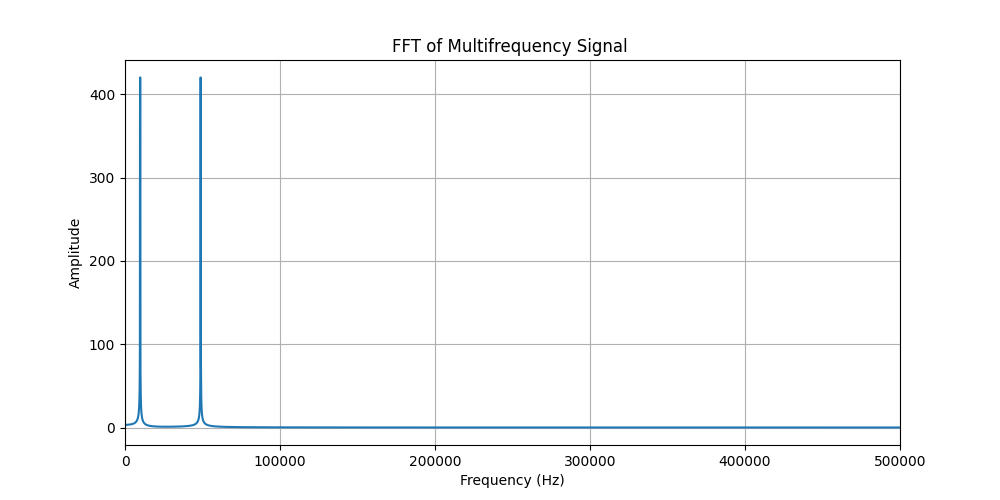
\includegraphics[width=0.9\linewidth]{imagess/FFT_2f.png}
    \caption{FFT magnitude spectrum of the 2-frequency multisine.}
    \label{fig:fft_2freq}
\end{figure}

\paragraph{5-Frequency multisine signal}  
The 5-frequency multisine signal was designed with frequencies spanning from 10 kHz to 250 kHz. Table~\ref{tab:freq_5f_corrected} lists the original frequencies, their quantized equivalents based on FFT resolution, and the corresponding frequency bin indices.

\begin{table}[H]
    \centering
    \caption{Frequency components for the 5-frequency multisine}
    \label{tab:freq_5f_corrected}
    \begin{tabular}{|p{2cm}|p{4cm}|p{4cm}|p{3cm}|}
        \hline
        \textbf{Frequency No.} & \textbf{Original frequency (Hz)} & \textbf{Quantized frequency (Hz)} & \textbf{Frequency bin index} \\
        \hline
        1 & 10000.0000       & 9765.6250     & 10  \\
        \hline
        2 & 22360.6798       & 22460.9375    & 23  \\
        \hline
        3 & 50000.0000       & 49804.6875    & 51  \\
        \hline
        4 & 111803.3989      & 111328.1250   & 114 \\
        \hline
        5 & 249999.9999      & 250000.0000   & 234 \\
        \hline
    \end{tabular}
\end{table}
 Figure~\ref{fig:fft_6freq} shows  the FFT magnitude spectra for the 5 frequencies configuration. The five spectral peaks appear at the expected logarithmically spaced positions, demonstrating the algorithm’s ability to handle higher-order configurations while preserving spectral purity and avoiding intermodulation artifacts.
\begin{figure}[H]
    \centering
    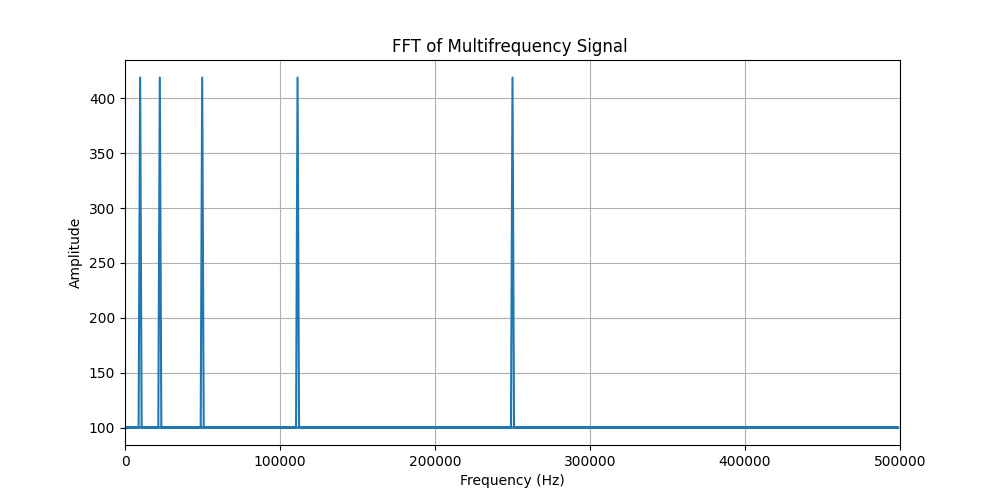
\includegraphics[width=0.9\linewidth]{imagess/FFT_5f.png}
    \caption{FFT magnitude spectrum of the 5-frequency multisine.}
    \label{fig:fft_6freq}
\end{figure}



\section{Experimental setup}
The experimental setup for validating the EIT system is shown in Figure~\ref{fig:setup}. The hardware consists of a Voltage-Controlled Current Source (VCCS) and the custom-designed EIT PCB connected to a circular tank equipped with 16 electrodes. The electrodes interface with the tissue-equivalent medium and allow current injection and voltage measurement.

The system is powered by a programmable laboratory power supply and monitored through a digital oscilloscope, which was used to visualize the injected multi-frequency waveforms and the corresponding electrode voltages. Data acquisition and communication with the microcontroller are carried out through a serial interface, with measurements logged using PuTTY on the host PC for further processing and reconstruction.

This configuration enabled simultaneous verification of the hardware signals (in time and frequency domains) and the digital acquisition pipeline, providing a complete validation of the EIT measurement chain from current injection to data recording.
\begin{figure}[H]
    \centering
    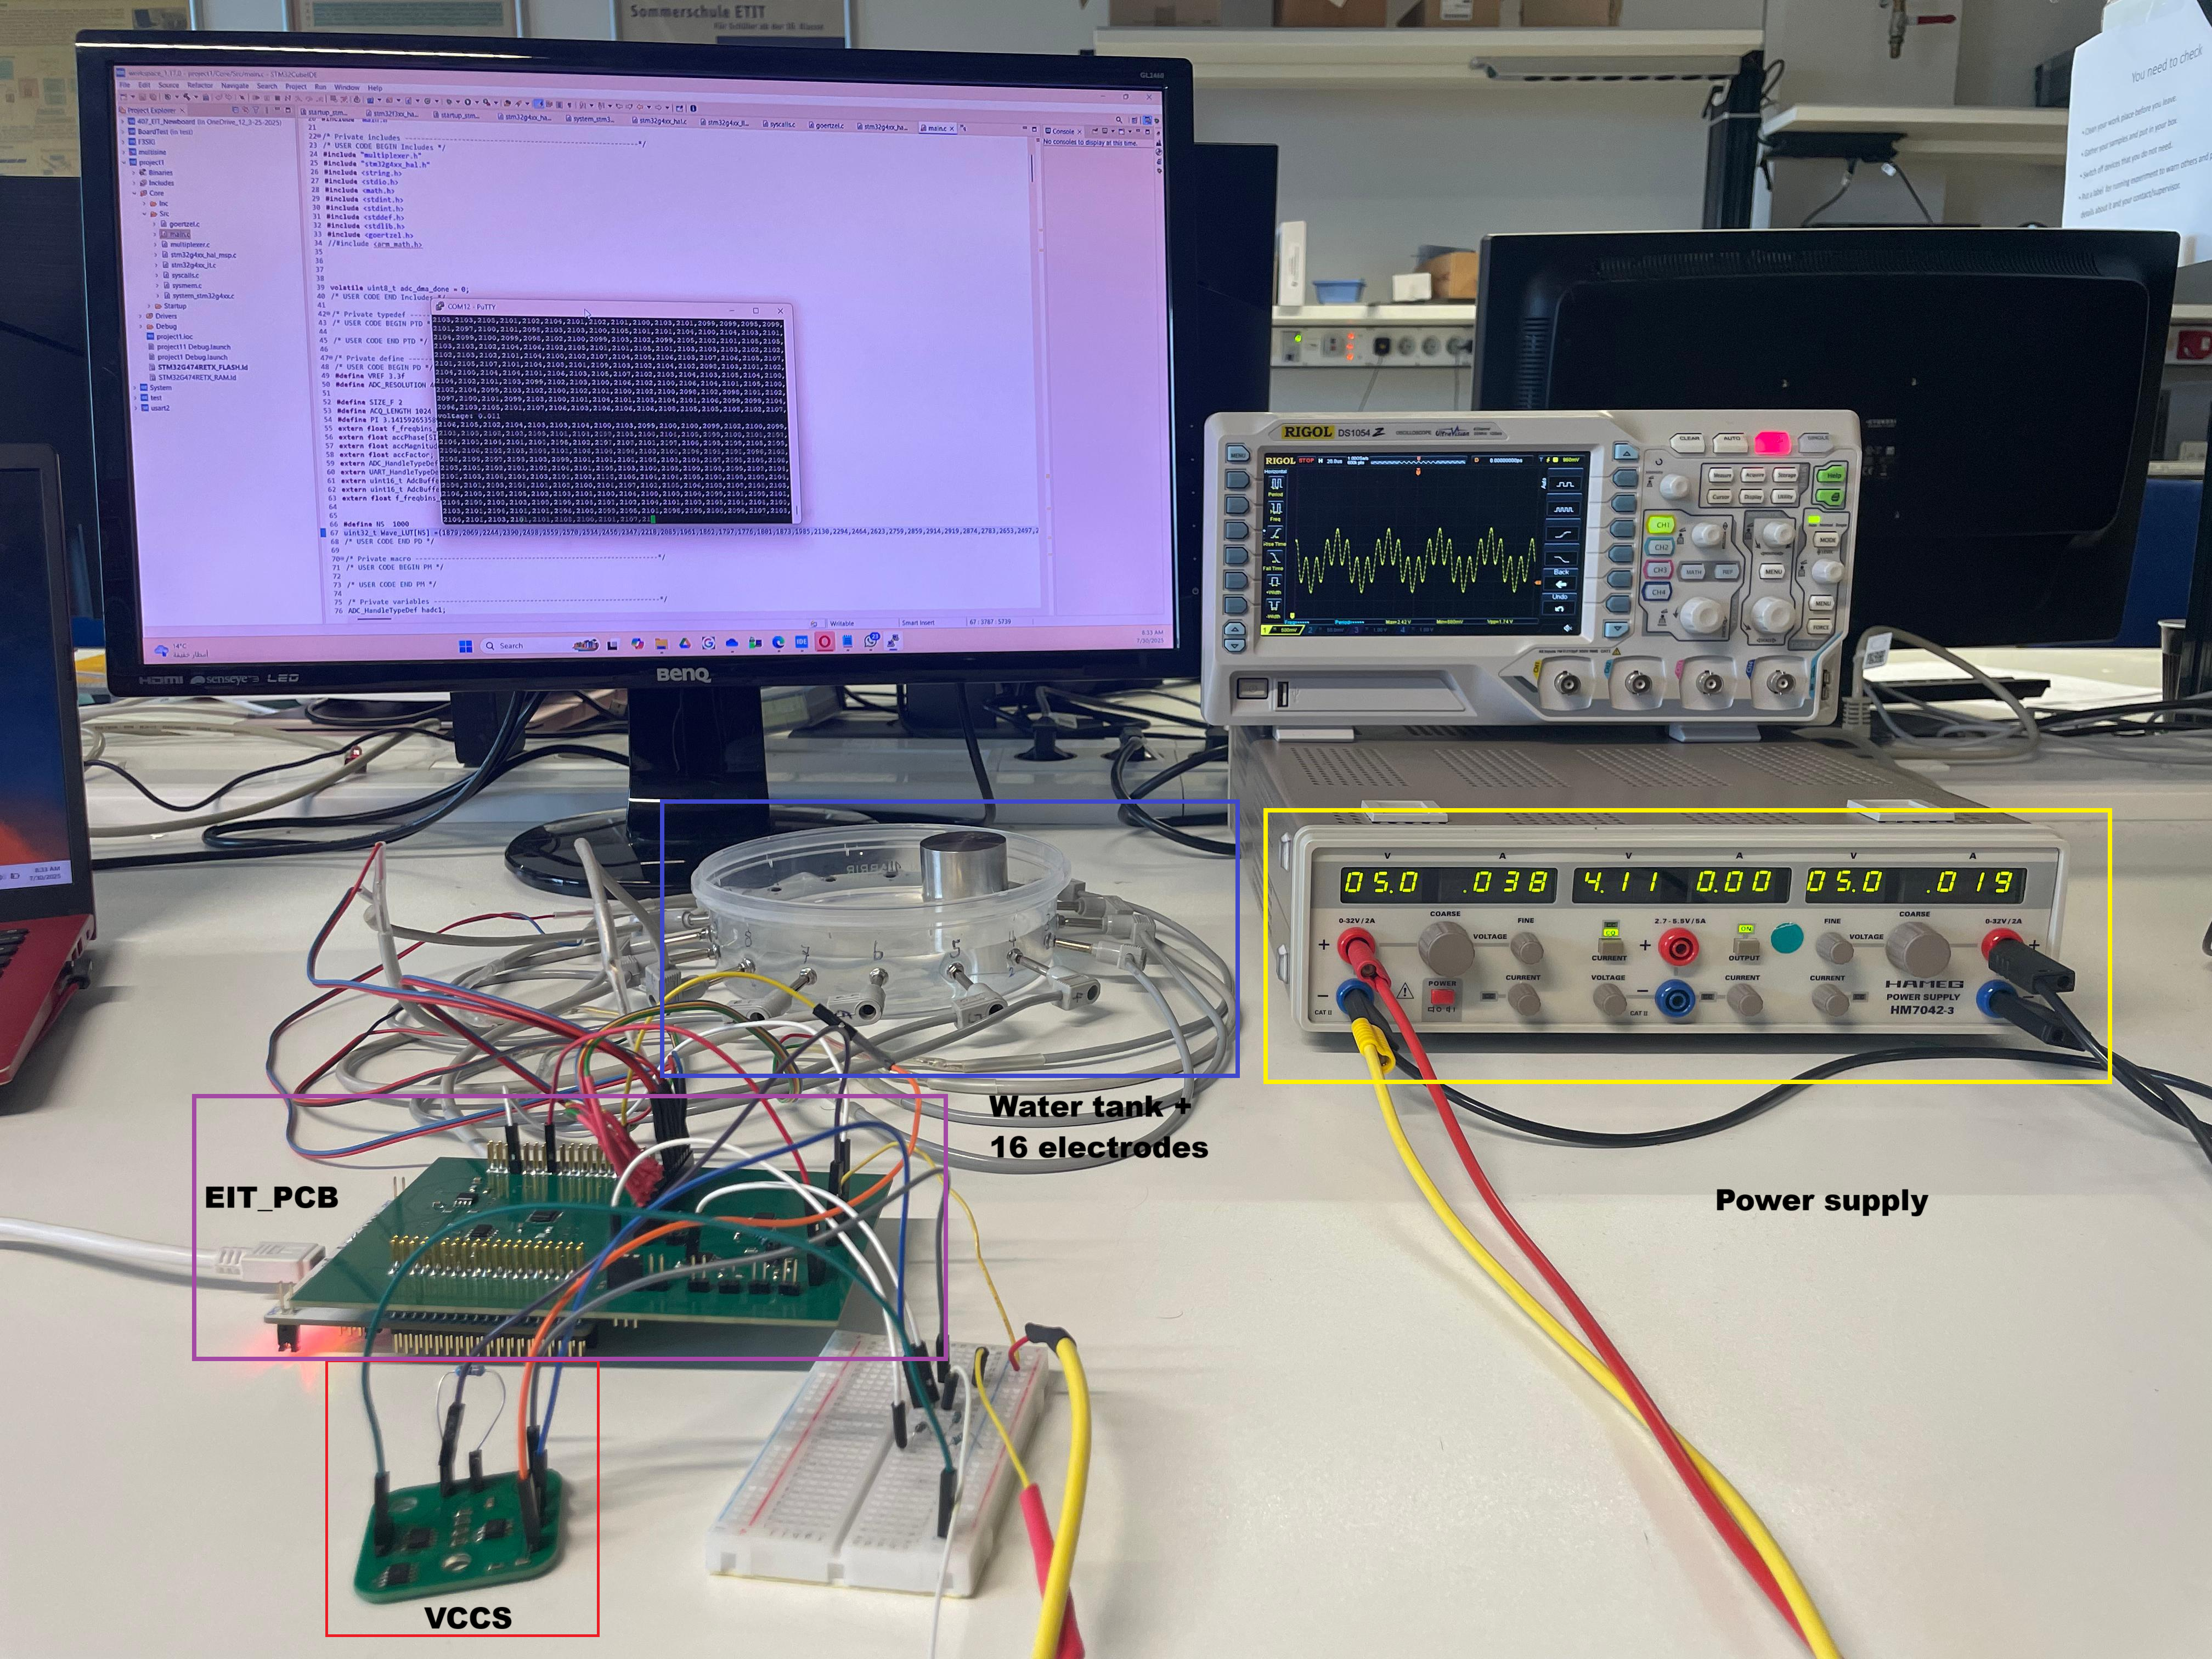
\includegraphics[width=0.95\textwidth]{imagess/setup.jpg}
    \caption{Experimental setup for system validation.}
    \label{fig:setup}
\end{figure}


\section{PCB testing and validation}
Before applying advanced signal processing and image reconstruction methods, it was essential to validate the designed PCB and ensure its correct functionality. The validation consisted of two main steps: (i) testing the circuit using a known resistance under monofrequency excitation, and (ii) testing the system with multi-frequency excitation using a water tank. These experiments demonstrate both the accuracy of the hardware and the robustness of the signal acquisition chain.  

\subsection{Validation with a known resistance}
To validate the analog front-end and switching architecture, the system was first tested by connecting a known resistor between two electrodes. A monofrequency sinusoidal excitation was injected by forcing the four multiplexers to select a pair of current-injection electrodes and a pair of voltage-sensing electrodes.  
 

The injected current and measured voltage were visualized on an oscilloscope. The calculated resistance, obtained from the ratio of measured voltage to current, closely matched the reference resistance value, confirming the accuracy of the measurement chain. Figure~\ref{fig:pcb_res_test} illustrates the oscilloscope visualization during this test.  

\begin{figure}[H]
    \centering
    \begin{subfigure}[b]{0.45\textwidth}
        \centering
        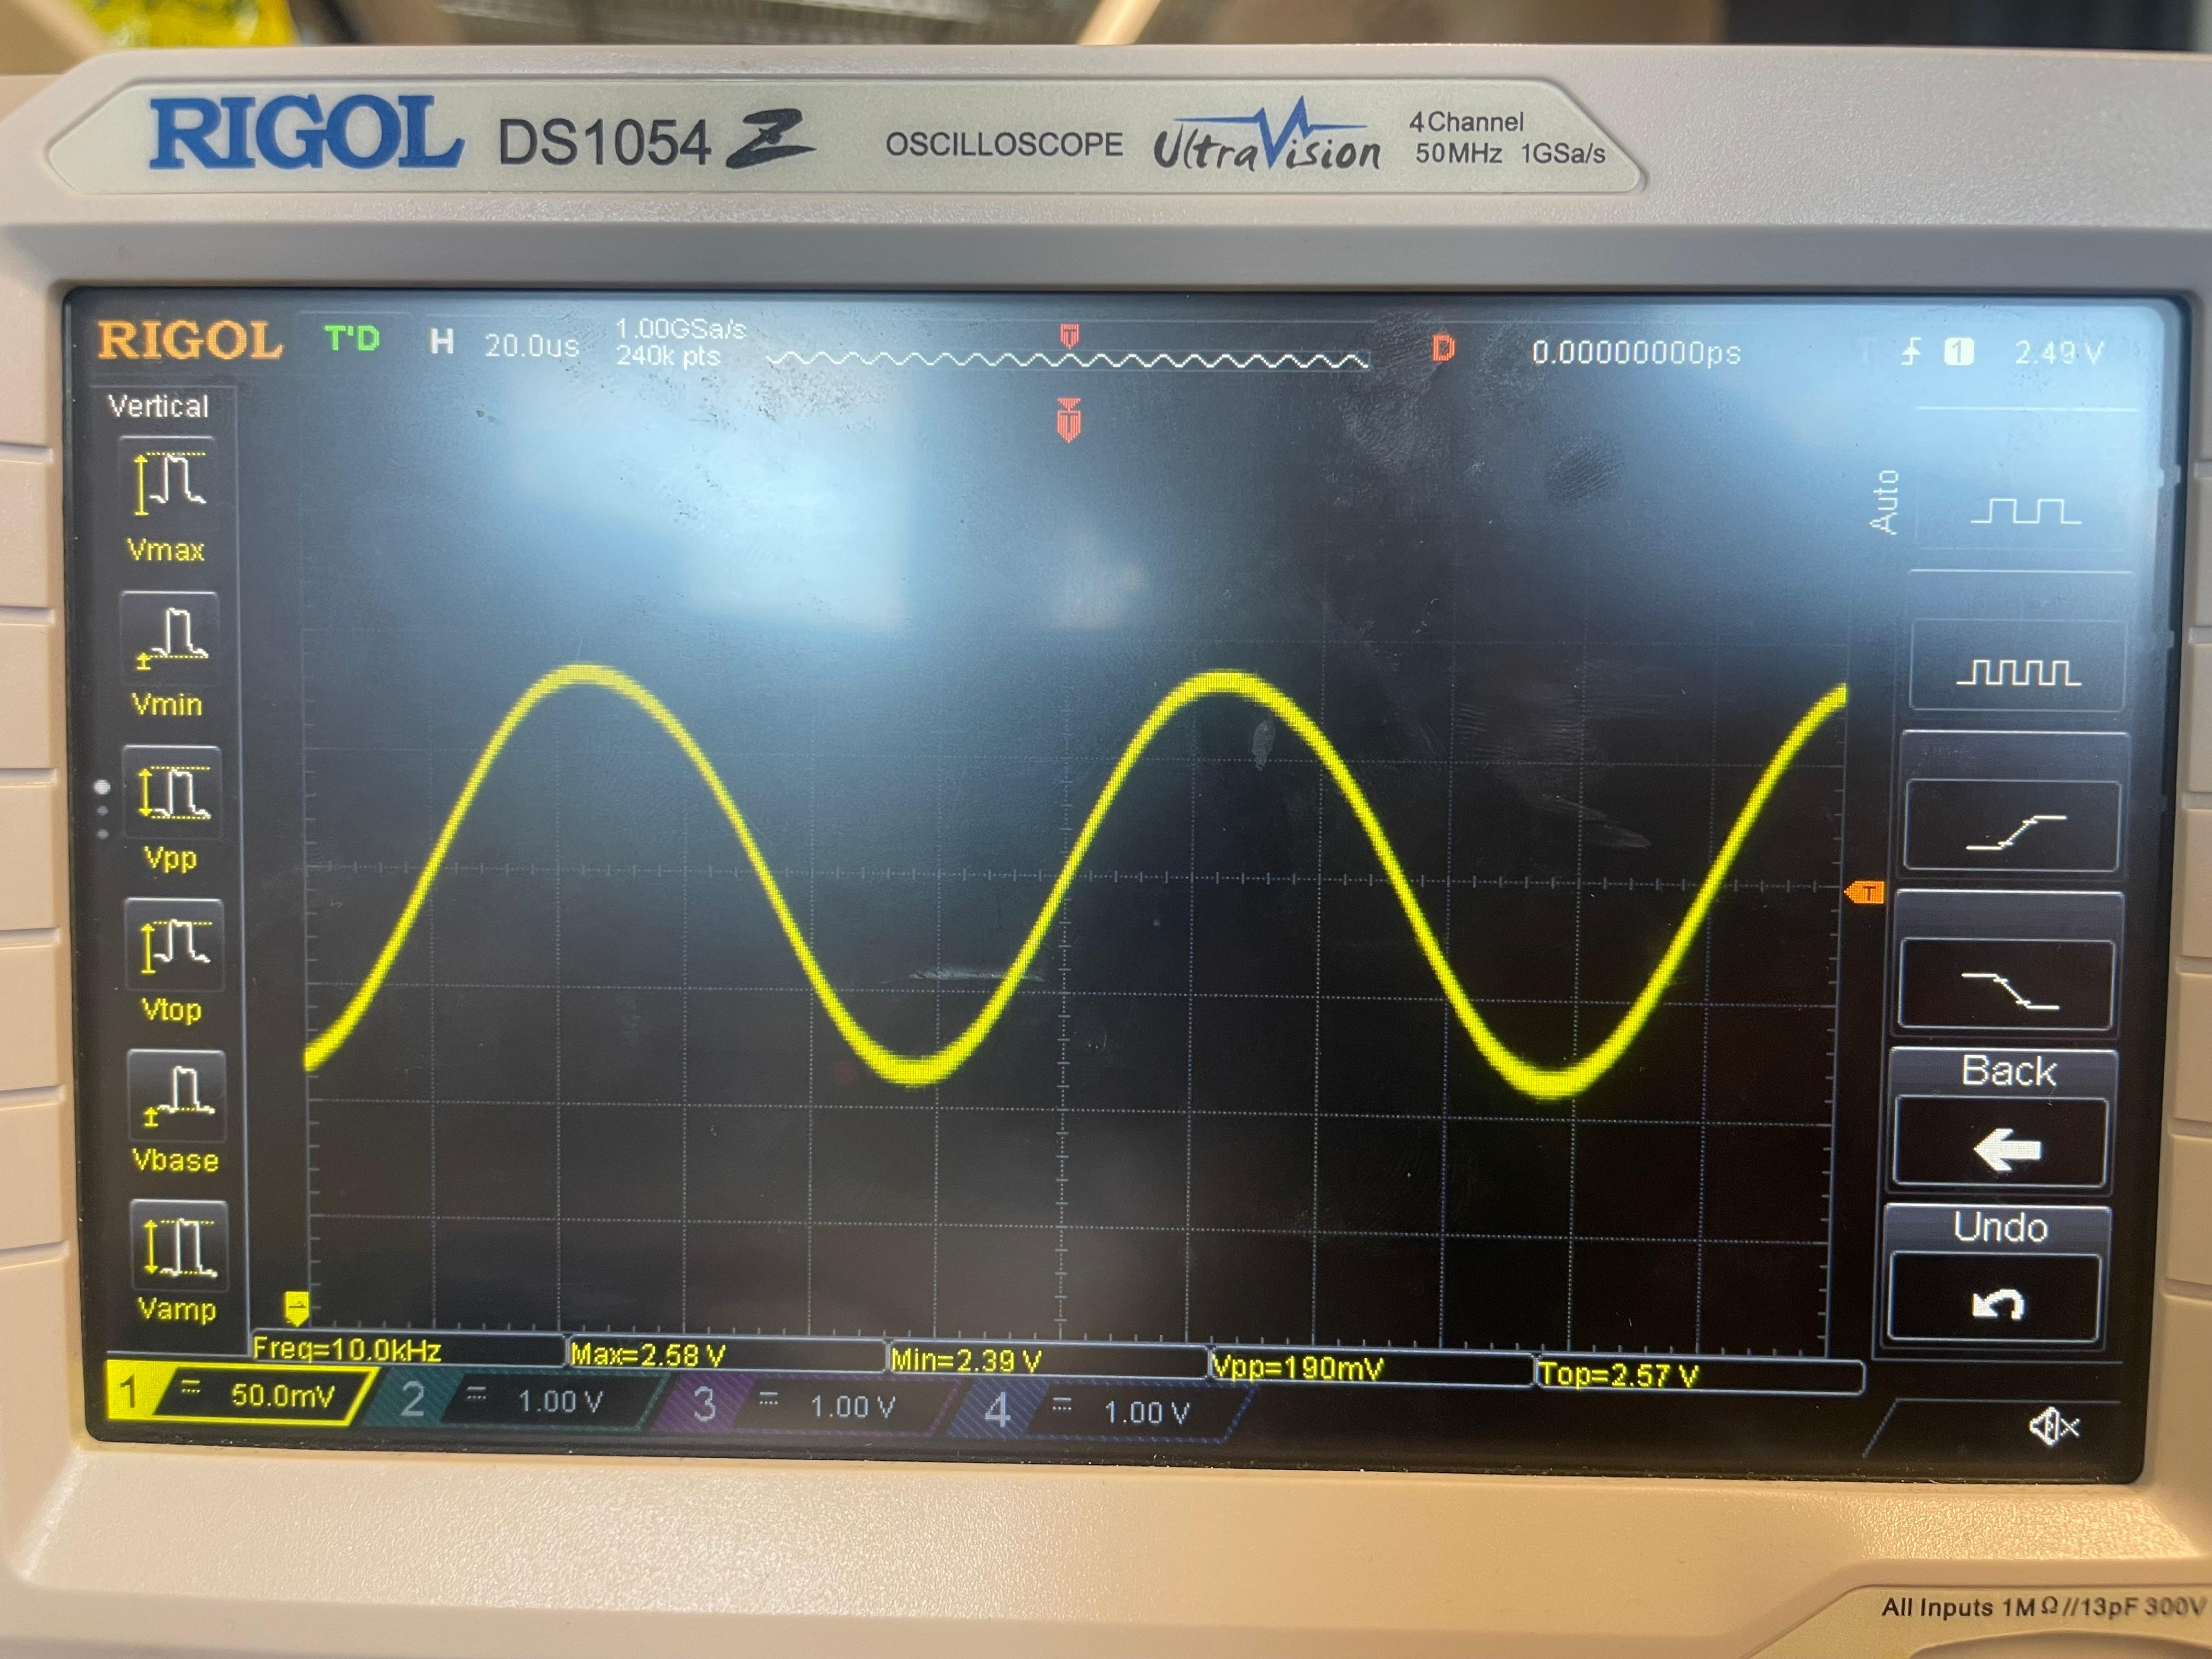
\includegraphics[width=\textwidth]{imagess/current.jpg}
        \caption{Measured current across a known resistance}
        \label{fig:current_test}
    \end{subfigure}
    \hfill
    \begin{subfigure}[b]{0.45\textwidth}
        \centering
        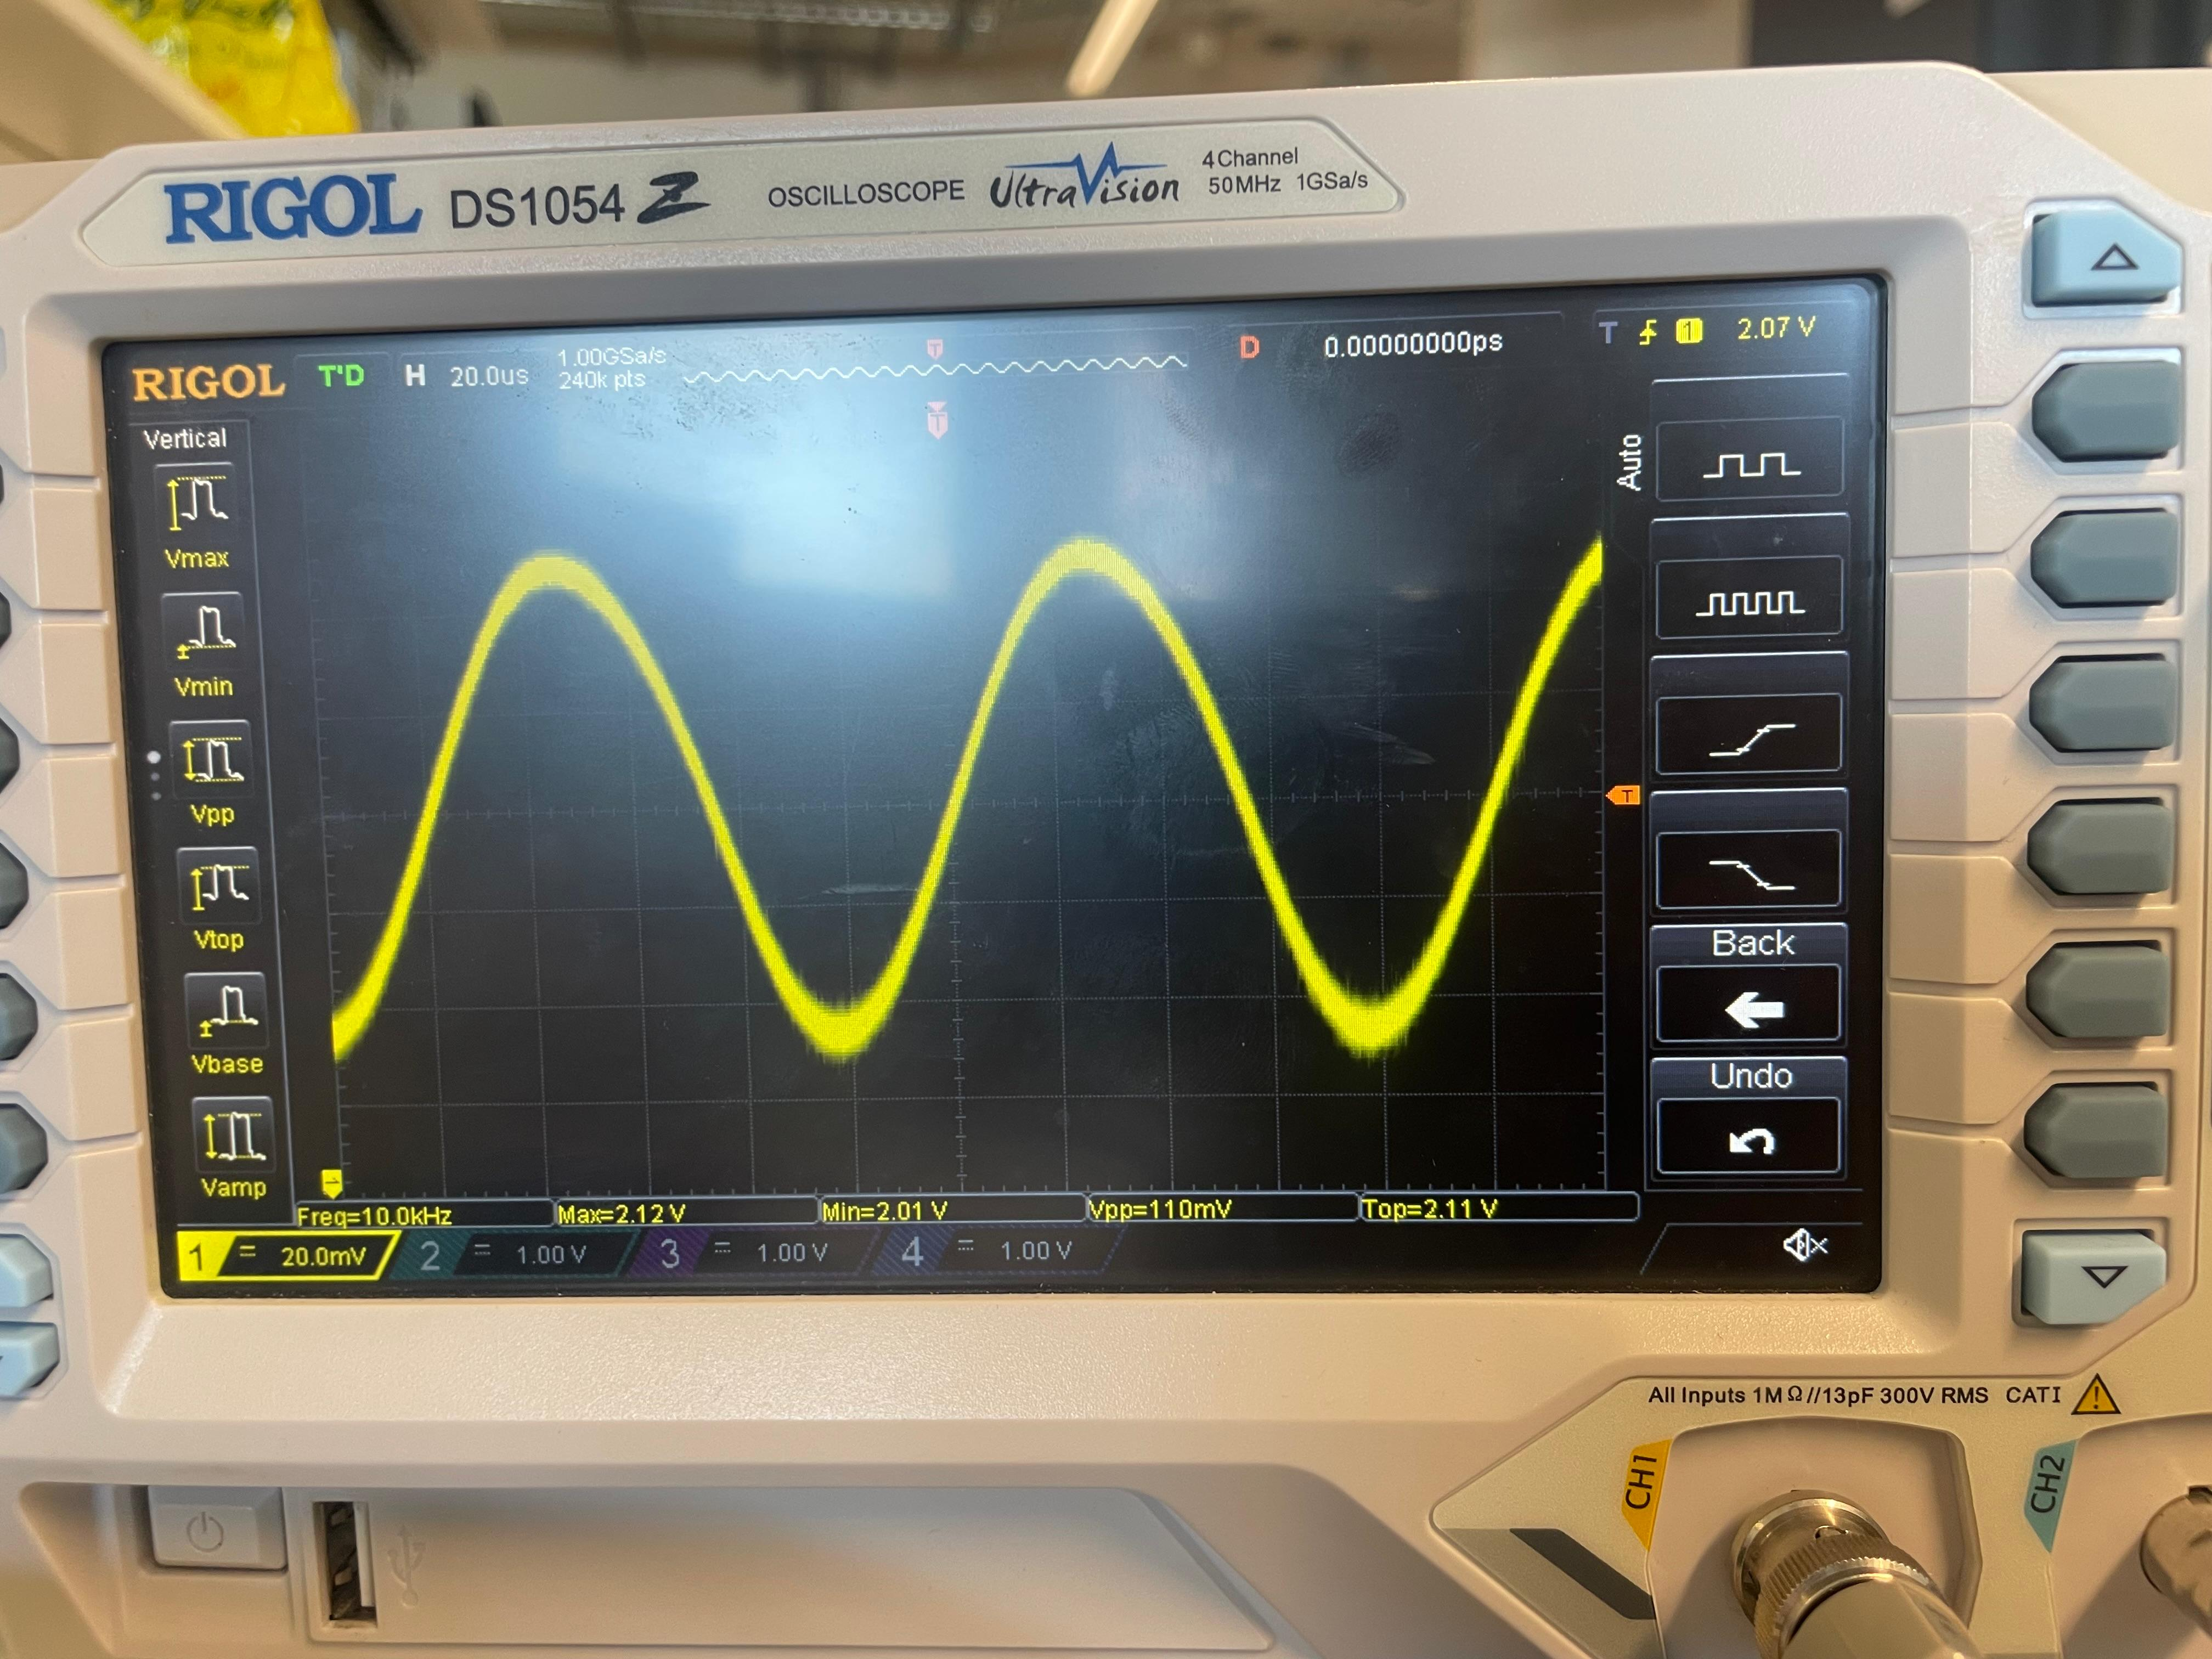
\includegraphics[width=\textwidth]{imagess/voltage.jpg}
        \caption{Measured voltage across a known resistance}
        \label{fig:voltage_test}
    \end{subfigure}
    \caption{Oscilloscope visualizations of the system response during a known resistance test.}
    \label{fig:pcb_res_test}
\end{figure}

Beyond qualitative waveform visualization, the system was quantitatively validated by extracting the peak-to-peak (V\textsubscript{pp}) values of the measured voltage and current signals from the oscilloscope traces.  

The procedure was as follows:  

\begin{itemize}

    \item The oscilloscope was used to measure the peak-to-peak voltage $V_{\text{pp,voltage}}$ across the load and the peak-to-peak voltage $V_{\text{pp,shunt}}$ across the current-sensing resistor $R_{\text{shunt}}$.
    \item The peak-to-peak current $I_{\text{pp}}$ was then calculated as:
    \begin{equation}
        I_{\text{pp}} = \frac{V_{\text{pp,shunt}}}{R_{\text{shunt}}}
    \end{equation}
    \item The load resistance $R_{\text{meas}}$ was obtained as:
    \begin{equation}
        R_{\text{meas}} = \frac{V_{\text{pp,voltage}}}{I_{\text{pp}}}
    \end{equation}
\end{itemize}

Table~\ref{tab:res_validation} summarizes the measured values compared with the true resistance ($\SI{1}{\kilo\ohm}$). The calculated resistance is in close agreement with the reference value, confirming the accuracy of the measurement chain.  

\begin{table}[H]
    \centering
    \caption{Oscilloscope-based validation of resistance measurement.}
    \label{tab:res_validation}
    \begin{tabular}{|c|c|c|c|c|}
        \hline
        $V_{\text{pp,voltage}}$ (mV) & $V_{\text{pp,shunt}}$ (mV) & $R_{\text{shunt}}$ ($\Omega$) & $I_{\text{pp}}$($\mu\text{A}$) & $R_{\text{meas}}$ ($\Omega$) \\
        \hline
       110 & 190 & 1000 & 190 & 578 \\
        \hline
    \end{tabular}
\end{table}
\subsection{Fabricated PCB after soldering}
After completing the design and fabrication process, the printed circuit board (PCB) was assembled by soldering all the required components.Figure~\ref{fig:pcb_after_soldering} shows the top side:

\begin{figure}[H]
    \centering
    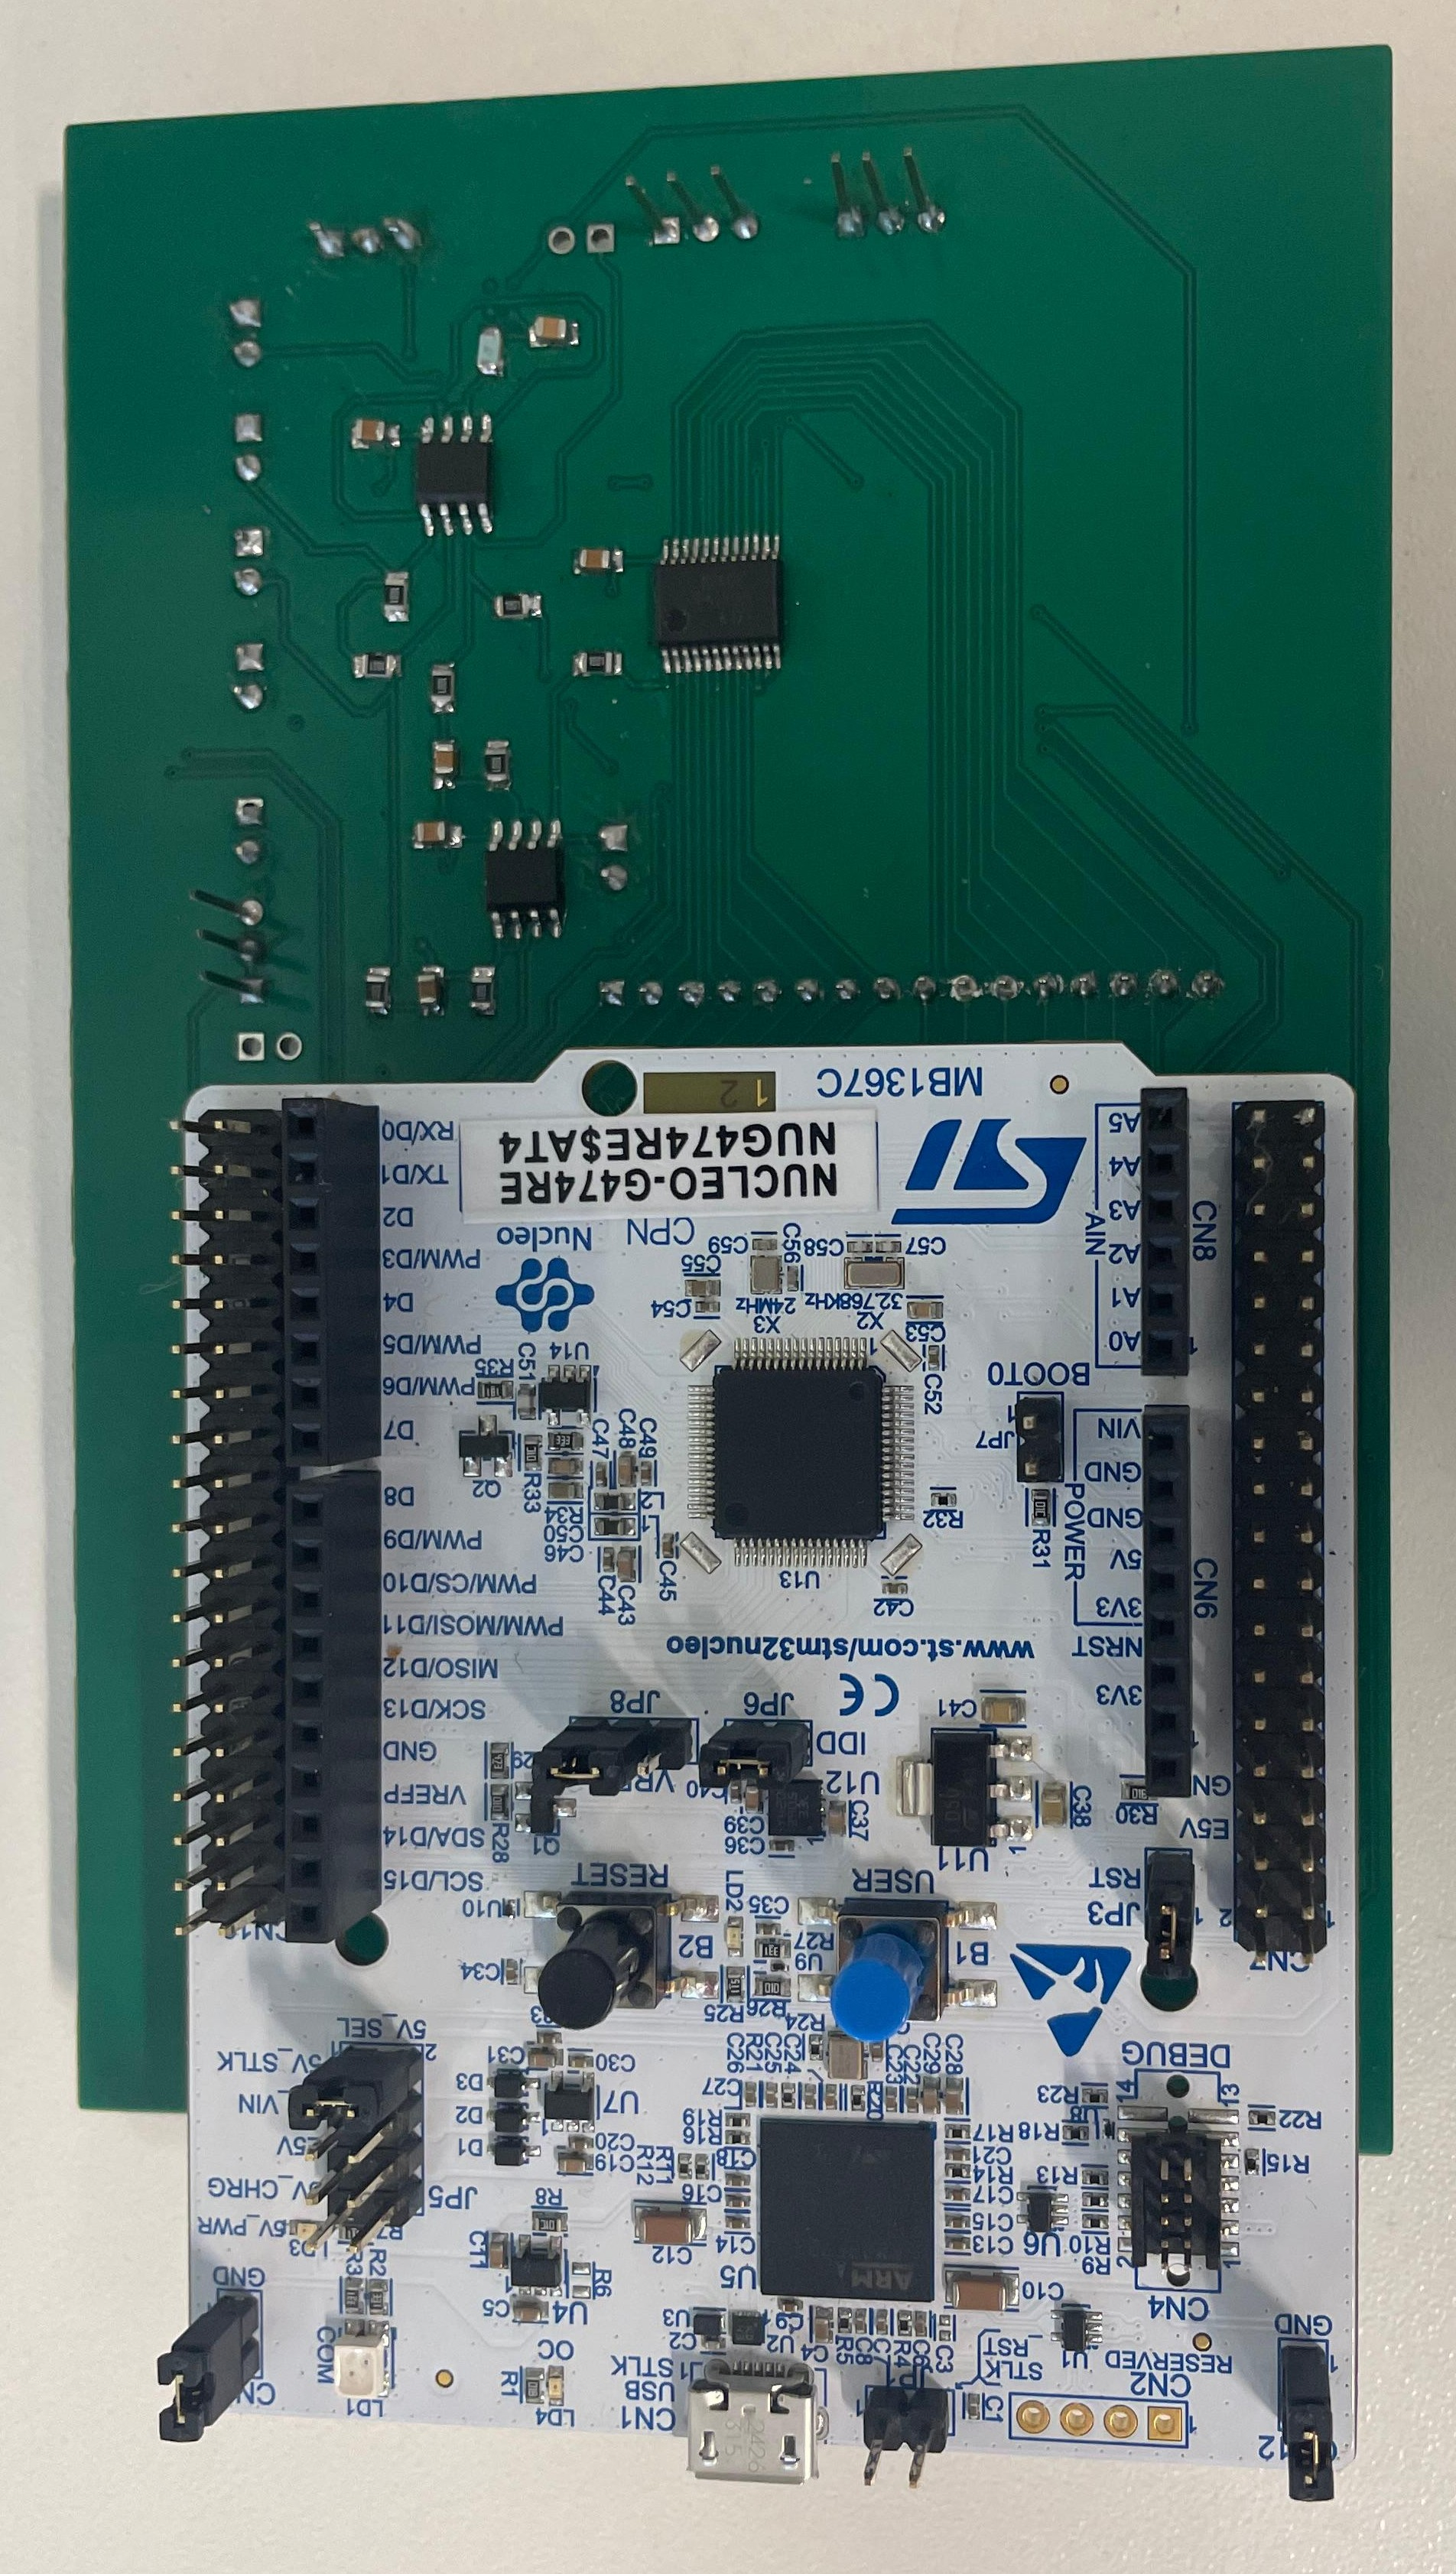
\includegraphics[width=0.65\textwidth]{imagess/top (1).jpg}
    \caption{Photograph of the fabricated PCB after soldering : top layer.}
    \label{fig:pcb_after_soldering}
\end{figure}
Figure~\ref{fig:pcb_after_soldering} shows the bottom side pf the PCB after soldering.
\begin{figure}[H]
    \centering
    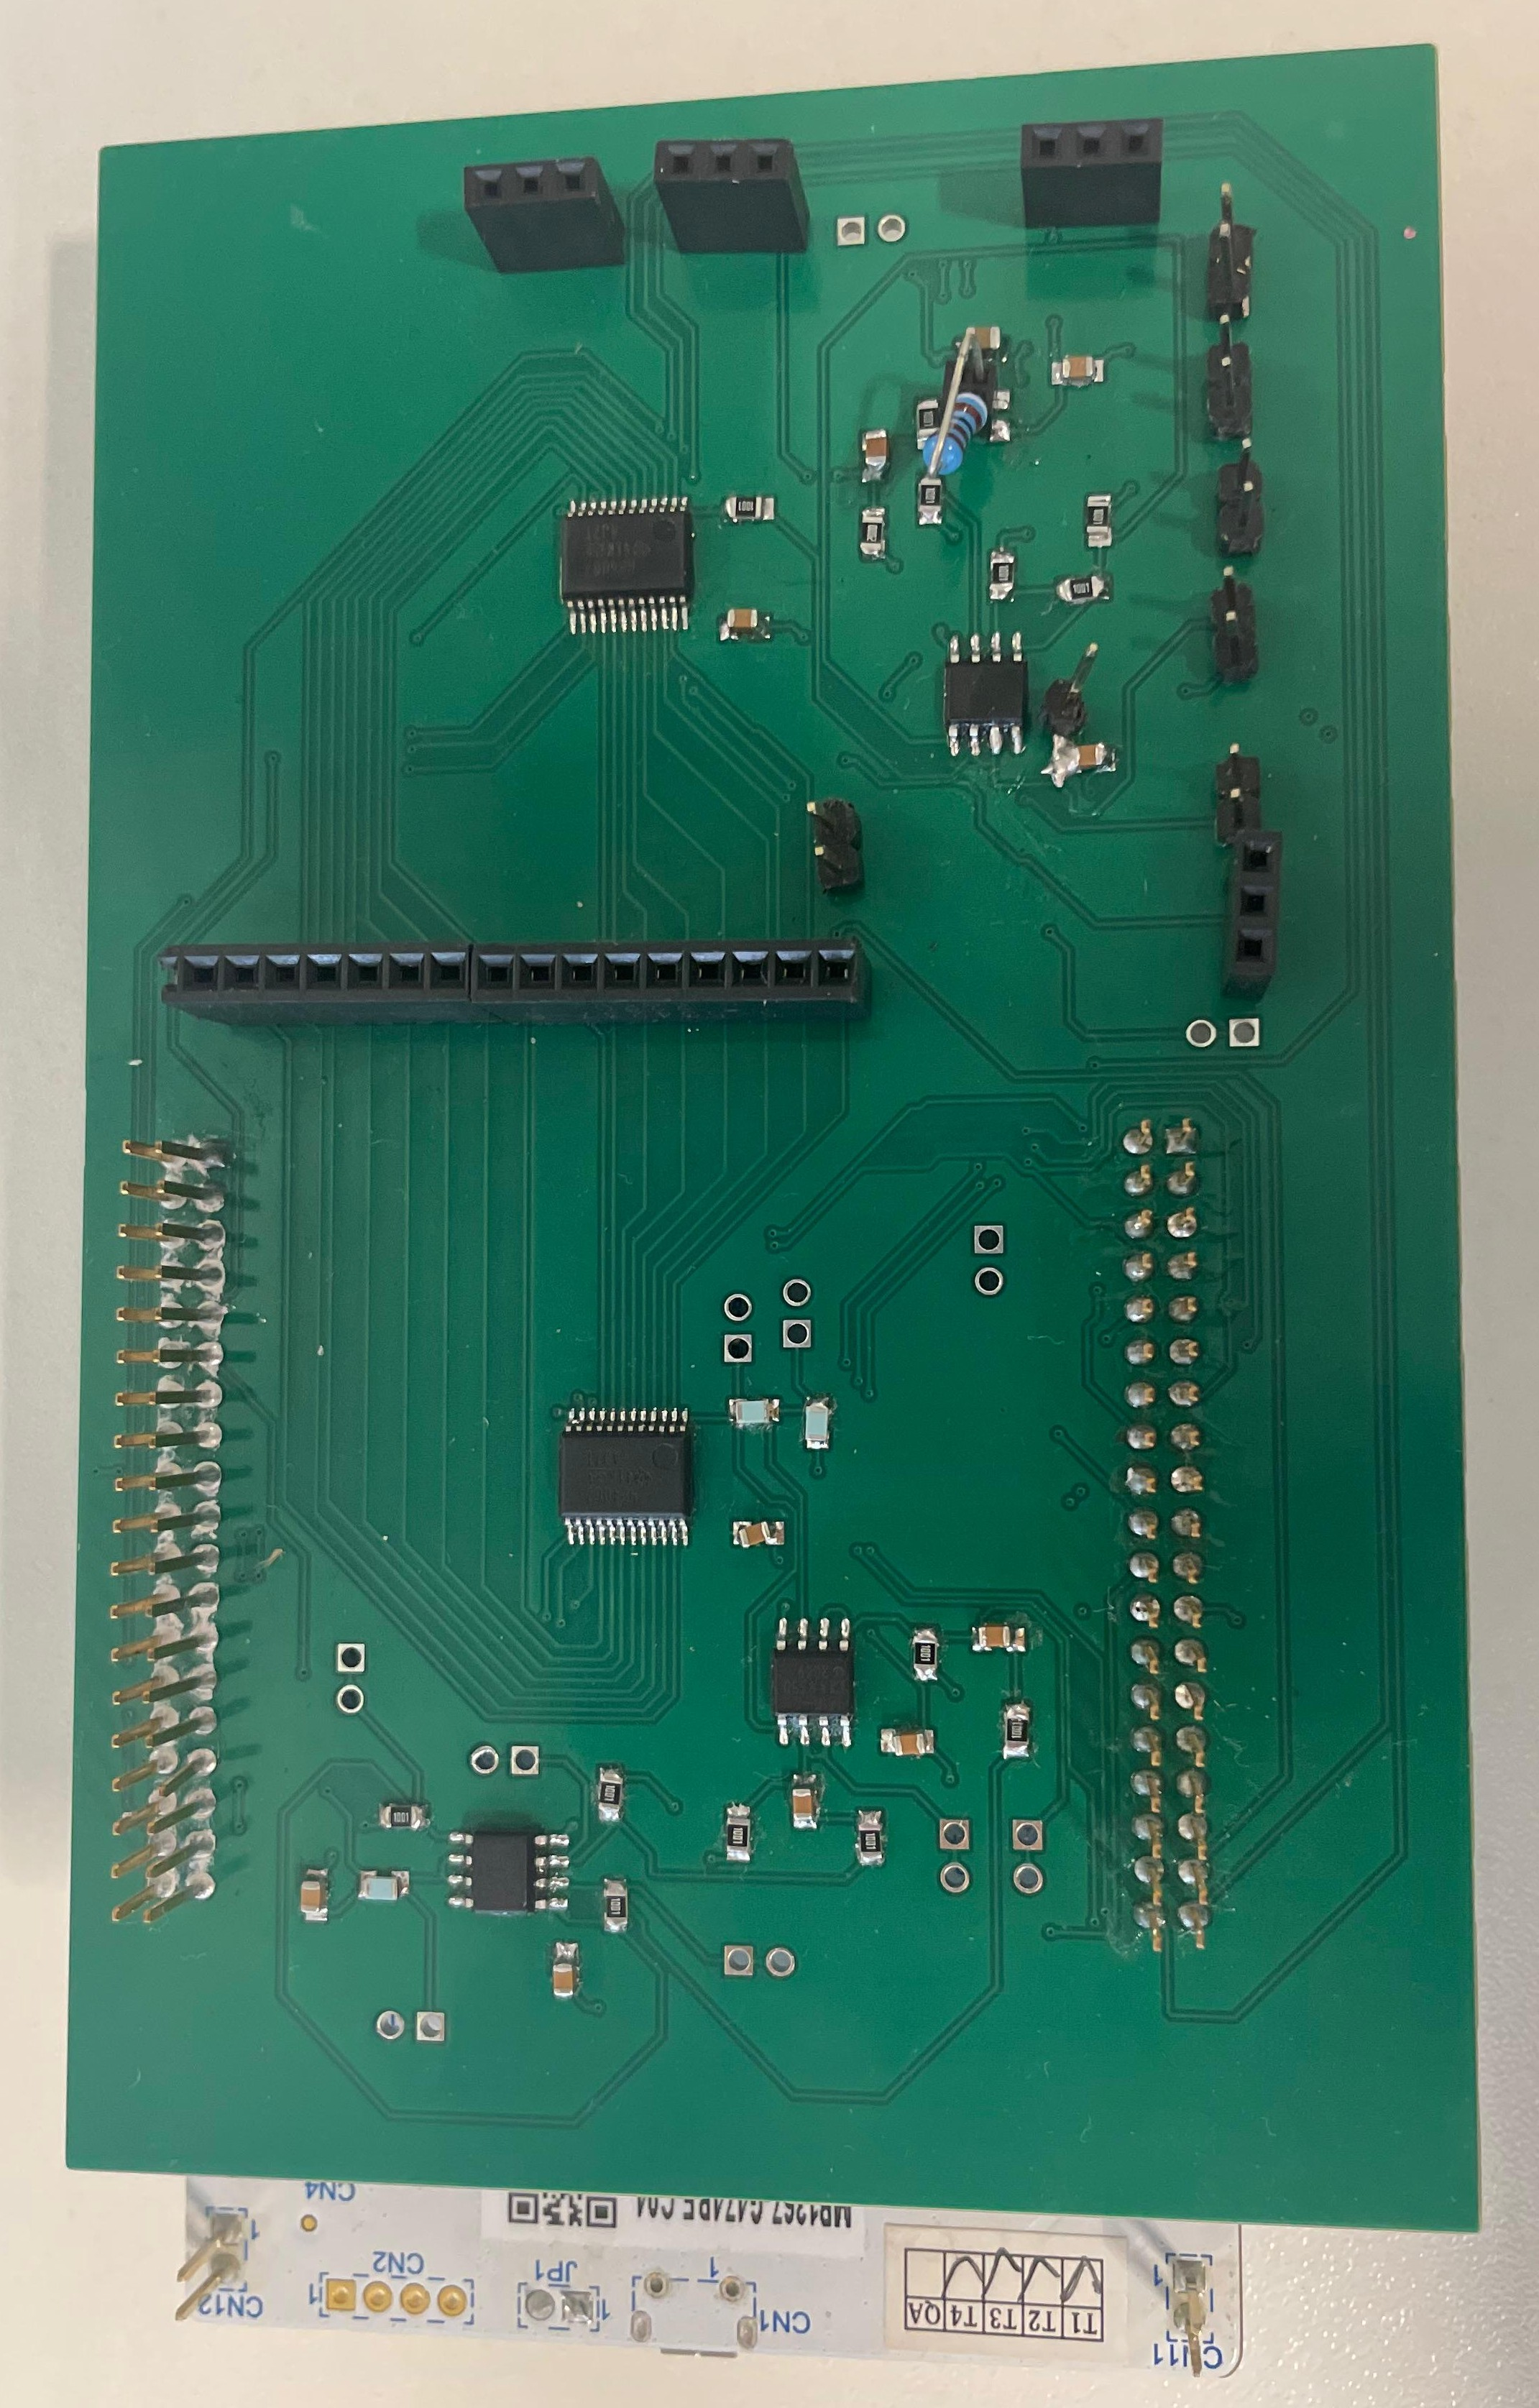
\includegraphics[width=0.65\textwidth]{imagess/bottom (1).jpg}
    \caption{Photograph of the fabricated PCB after soldering : bottom layer.}
    \label{fig:pcb_after_soldering}
\end{figure}

\section{Frequency-domain validation across 2 excitation frequencies}

To quantitatively validate the multi-frequency excitation, the system was tested with a known resistive load. 
The multiplexer was fixed to inject current between two electrodes and measure voltage between two others. 
The raw ADC samples were processed using both the Fast Fourier Transform (FFT) and the Goertzel algorithm implemented in Python. 
This allowed direct extraction of the magnitudes at the excitation frequencies (9.765 ~kHz and 49.804~kHz).

\subsection{FFT-based validation}
Figures~\ref{fig:fft_current} and \ref{fig:fft_voltage} present the FFT spectra of the injected current and measured voltage, respectively. 
Two distinct peaks are clearly visible at 9765~Hz and 49804~Hz, confirming that the multi-frequency excitation is correctly generated and acquired.

\begin{figure}[H]
    \centering
    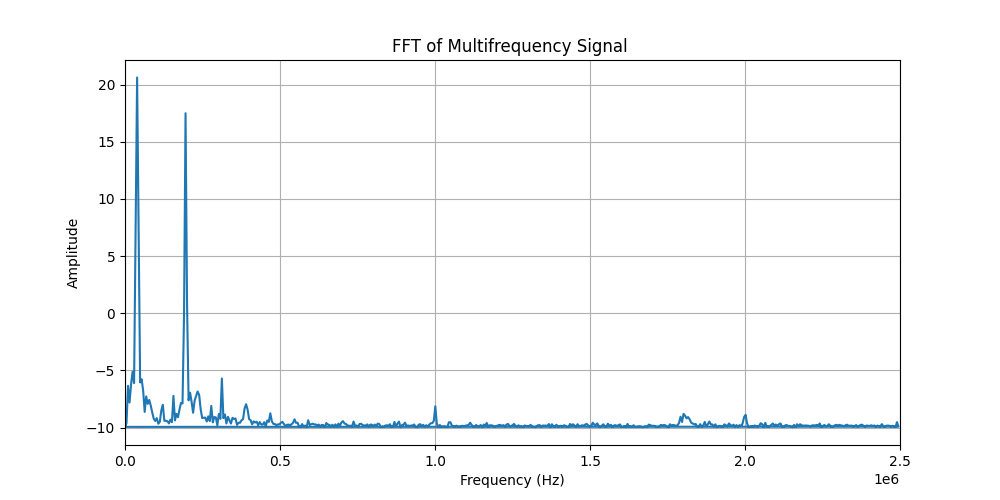
\includegraphics[width=0.85\textwidth]{imagess/Figure_current.png}
    \caption{FFT spectrum of the injected current showing distinct peaks at at $9765.6250$~Hz and   at $49804.6875$~Hz.}
    \label{fig:fft_current}
\end{figure}

\begin{figure}[H]
    \centering
    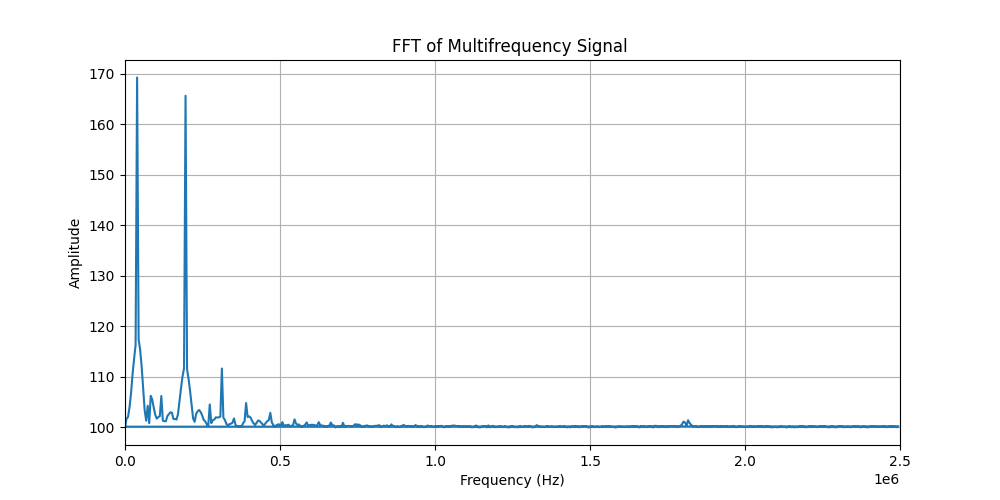
\includegraphics[width=0.85\textwidth]{imagess/fft2_measuredvoltage.png}
    \caption{FFT spectrum of the measured voltage showing distinct peaks at $9765.6250$~Hz and   at $49804.6875$~Hz.}
    \label{fig:fft_voltage}
\end{figure}

From the FFT magnitude values, the ADC peaks at $9765.6250$~Hz were found to be approximately:  
\[
V_{\text{measured}} \approx 170 \ \text{ADC counts}, 
\qquad V_{\text{shunt}} \approx 21 \ \text{ADC counts}.
\]

With a 12-bit ADC ($4096$ levels) and $V_{\mathrm{ref}}=3.3$~V, this corresponds to:
\[
V_{\mathrm{meas}}=\frac{170}{4096}\cdot 3.3 \approx 0.137~\text{V}, \qquad
V_{\mathrm{shunt}}=\frac{21}{4096}\cdot 3.3 \approx 0.0169~\text{V}.
\]

Using a shunt resistor of $R_{\mathrm{shunt}}=70~\Omega$, the injected current is:
\[
I = \frac{V_{\mathrm{shunt}}}{R_{\mathrm{shunt}}} = \frac{0.0169}{70} \approx 0.241~\text{mA}.
\]

The equivalent load resistance is therefore:
\[
R_{\mathrm{meas}} = \frac{V_{\mathrm{meas}}}{I} = \frac{0.137}{0.241\times 10^{-3}} \approx 568~\Omega,
\]
which is in good agreement with the true load value of $600~\Omega$.  
At $49804.6875$~Hz $R_{mes} = 637.995~\Omega$, confirming the frequency-independent behavior and the accuracy of the acquisition chain.

To further validate the results, the Goertzel algorithm was implemented in Python and applied to the same ADC datasets. 
The extracted magnitudes of voltage and current at 10~kHz and 50~kHz led to resistance values very close to those obtained with the FFT method. 
This demonstrates that both spectral techniques provide consistent and reliable results for impedance extraction in multi-frequency EIT.
\subsection{Quantitative evaluation of FFT-based validation}

To complement the qualitative observation of the FFT spectra, we quantified the accuracy of the impedance estimation at both excitation frequencies. The equivalent resistance was extracted from the ratio of measured voltage to current and compared to the known reference load of $600~\Omega$. The relative error was computed using:

\begin{equation}
\text{Error}(\%) = \frac{|R_{\text{measured}} - R_{\text{reference}}|}{R_{\text{reference}}} \times 100
\end{equation}

Table~\ref{tab:fft_eval} summarizes the results obtained with the FFT-based approach.

\begin{table}[H]
\centering
\caption{FFT-based resistance estimation and error analysis for two-frequency excitation}
\label{tab:fft_eval}
\begin{tabular}{|c|p{4cm}|p{4cm}|c|}
\hline
\textbf{Frequency (Hz)} & \textbf{Reference Resistance ($\Omega$)} & \textbf{Measured Resistance ($\Omega$)} & \textbf{Error (\%)} \\ \hline
9765.625  & 600 & 568   & 5.3  \\ \hline
49804.687 & 600 & 638   & 6.3  \\ \hline
\end{tabular}
\end{table}

The extracted resistance values closely match the true load, with errors below 7\%. This confirms that the proposed acquisition chain maintains reliable performance across both low and high excitation frequencies. 


\section{Validation of data acquisition and signal fidelity}
\label{sec:adc_validation}

Accurate acquisition of voltage measurements is a critical requirement for Electrical Impedance Tomography (EIT) systems. To ensure the reliability of the developed data acquisition system, the analog-to-digital converter (ADC) readings were validated using both mono- and multi-frequency excitation signals. This verification guarantees that the recorded impedance data accurately reflects the applied electrical stimuli, which is essential for subsequent tomographic reconstruction.

Figure~\ref{fig:adc_mono} shows the ADC readings obtained during a monofrequency excitation at 9.76 kHz. The acquired waveform closely follows the expected sinusoidal signal, indicating proper operation of the ADC and the signal conditioning circuitry.

\begin{figure}[H]
    \centering
    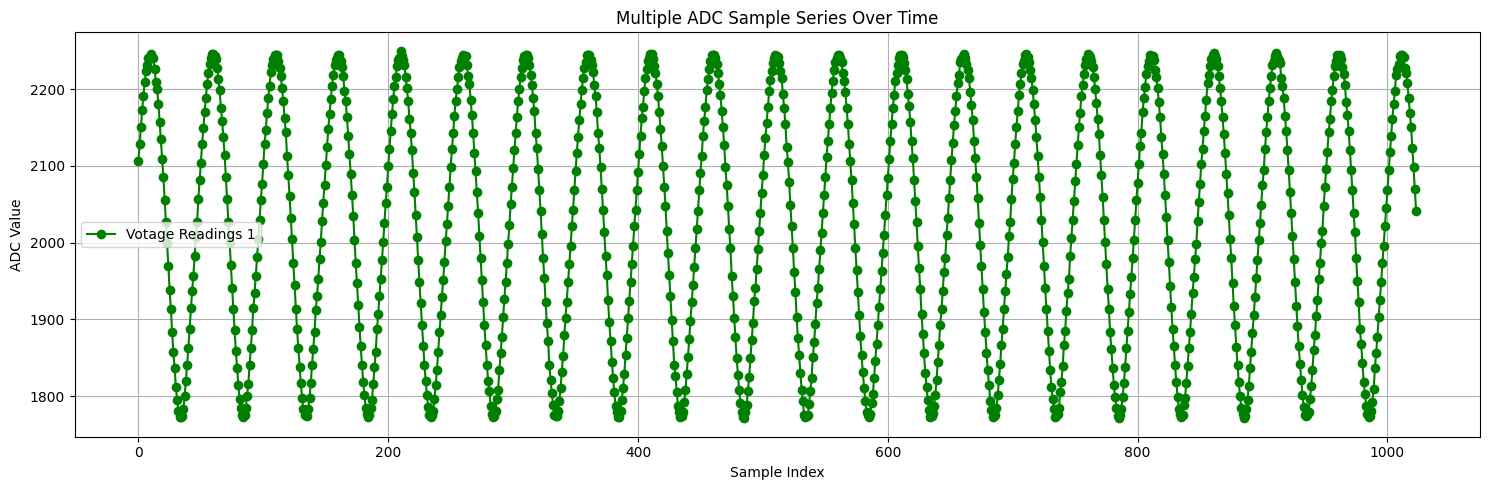
\includegraphics[width=0.8\textwidth]{imagess/s1.png}
    \caption{ADC readings for monofrequency excitation at 9.76 kHz. The waveform demonstrates accurate and stable sampling across multiple trials.}
    \label{fig:adc_mono}
\end{figure}

To further assess the system under realistic measurement conditions, multi-frequency excitation signals were applied, combining 9.76 kHz and 49.80 kHz components. Figure~\ref{fig:adc_multi} presents the corresponding ADC readings. The superimposed waveforms confirm that the ADC captures the composite signal with high fidelity, preserving both frequency components without noticeable distortion. This demonstrates that the system can reliably acquire data for multi-frequency EIT measurements, which are crucial for enhanced imaging sensitivity and resolution.

\begin{figure}[H]
    \centering
    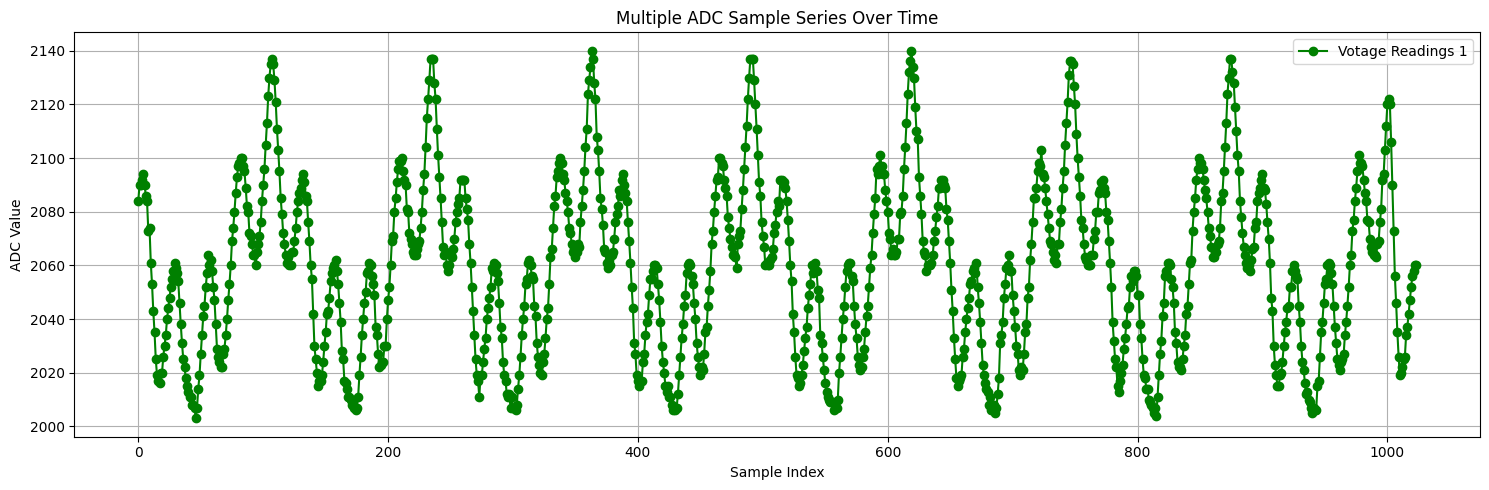
\includegraphics[width=0.8\textwidth]{imagess/s2.png}
    \caption{ADC readings for multi-frequency excitation at 9.76 kHz and 49.80 kHz. The ADC correctly resolves both frequency components, confirming signal fidelity.}
    \label{fig:adc_multi}
\end{figure}

The results from both monofrequency and multi-frequency validations confirm that the ADC and the associated acquisition pipeline provide accurate, stable, and repeatable measurements. These validations serve as a foundation for the reproducibility analyses presented in the next Sections.

\section{Measurement reproducibility across 2 excitation frequencies}
To ensure the reliability of the developed EIT acquisition system, it is important to
assess how consistently the measurements can be reproduced under repeated trials
and across different excitation frequencies. This section presents an experimental
evaluation of reproducibility, by comparing results at two representative
frequencies.
The following figures show the impedance variation over 20 trials for two different frequencies. The data was processed using a Python script that performs the following steps:

\begin{enumerate}
    \item Reads the raw EIT measurement data for each trial.
    \item Applies the Goertzel algorithm to extract the signal component at the frequency of interest.
    \item Computes the impedance values from the measured signals.

    \item Generates plots of the impedance variation across the 208 measurements for each trial.
\end{enumerate}

These steps allow visualizing how the impedance changes over repeated trials and between the two frequencies under study.

\begin{figure}[H]
    \centering
    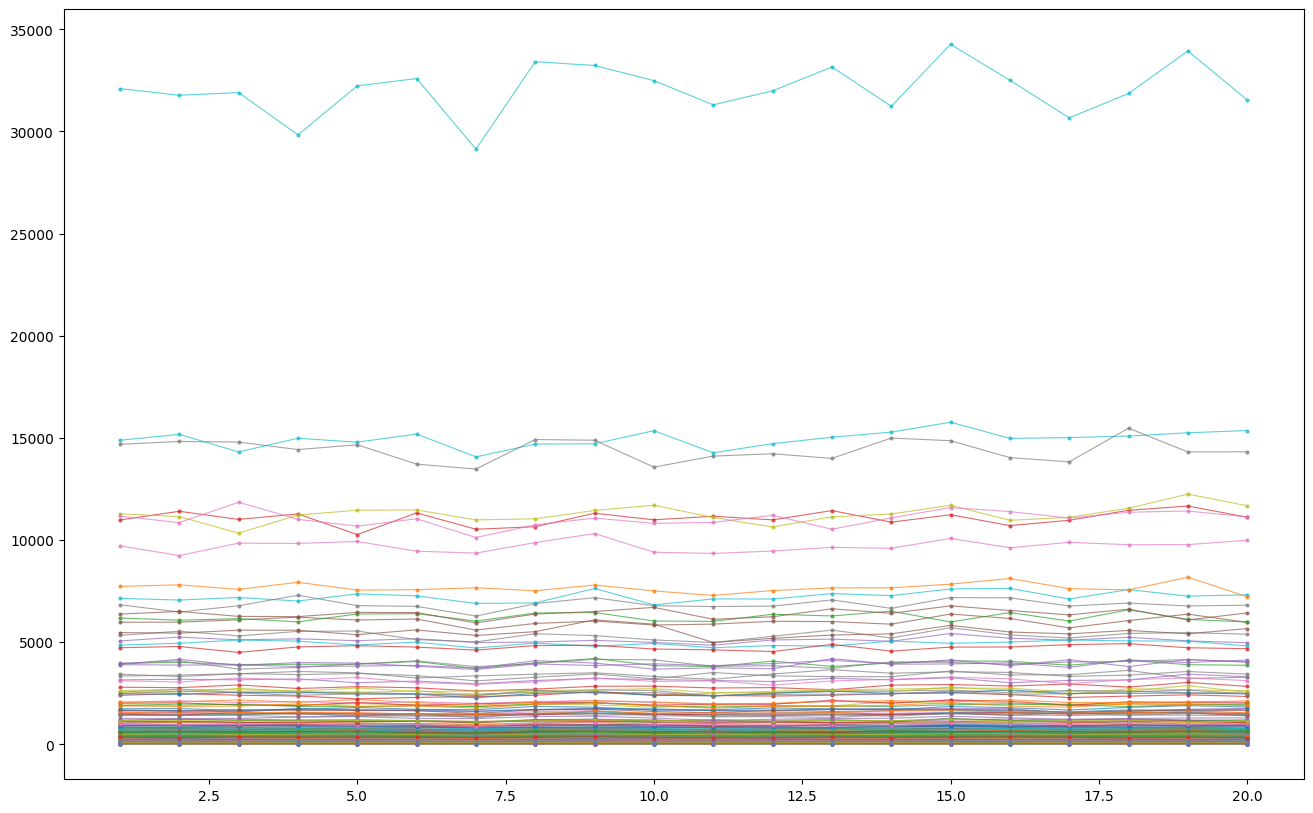
\includegraphics[width=0.7\textwidth]{imagess/2f_2.png}
    \caption{Impedance variation over 20 trials for \(f = 9765 \,\text{Hz}\) after Goertzel and impedance calculation.}
    \label{fig:stability_lowfreq}
\end{figure}

\begin{figure}[H]
    \centering
    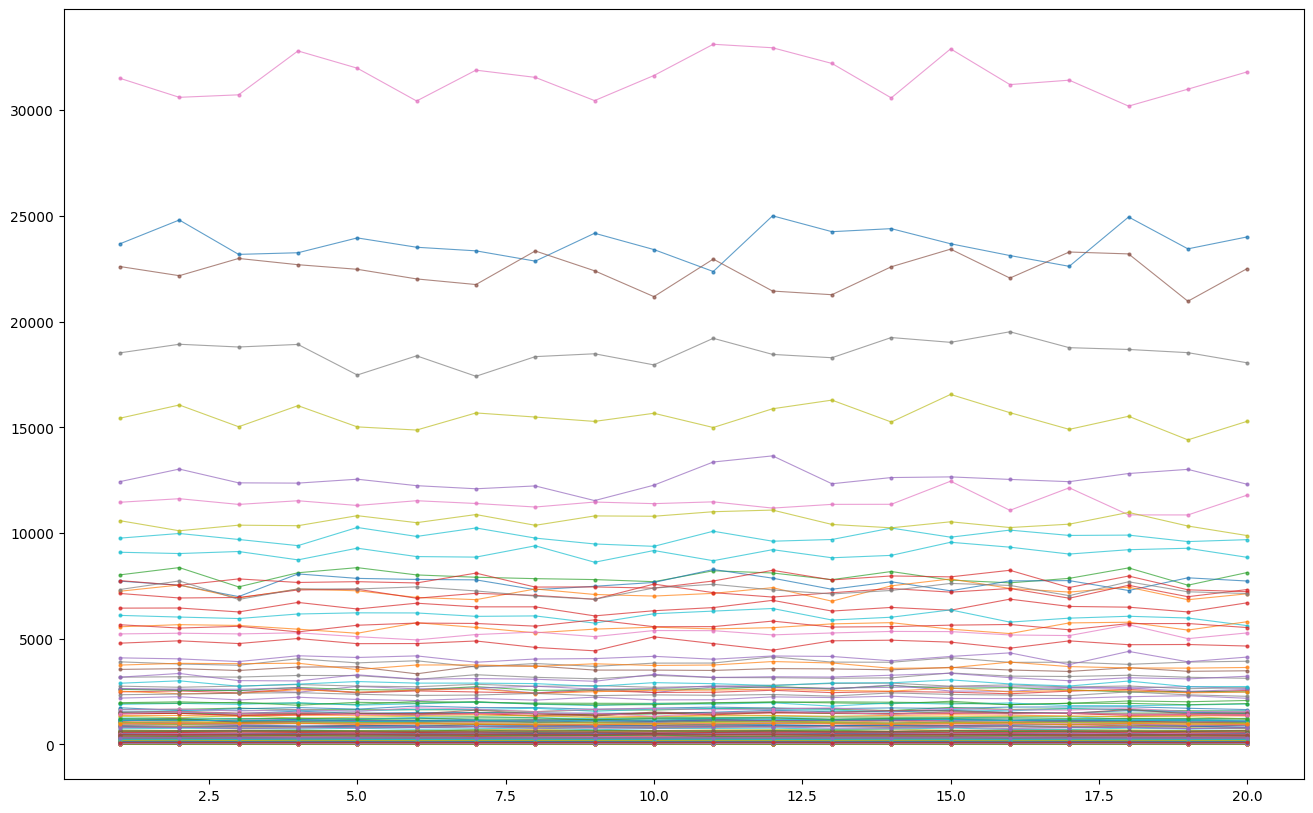
\includegraphics[width=0.7\textwidth]{imagess/2f_1.png}
    \caption{Impedance variation over 20 trials for \(f = 49804 \,\text{Hz}\) after Goertzel and impedance calculation.}
    \label{fig:stability_highfreq}
\end{figure}

The impedance results presented in Figures~\ref{fig:stability_lowfreq} and 
\ref{fig:stability_highfreq} confirm the robustness of the measurement system. 
For the lower frequency case (\(f = 9765 \,\text{Hz}\)), the impedance values 
remain highly stable across the 20 trials, with only minor fluctuations. 
This demonstrates that the system maintains a consistent response under 
repeated measurements.

At the higher frequency (\(f = 49804 \,\text{Hz}\)), the impedance curves 
exhibit slightly larger variations between trials, which can be attributed 
to increased sensitivity of the measurement to electrode-skin interface 
changes and parasitic effects at higher frequencies. Nevertheless, the 
overall trends remain consistent, indicating that the system does not suffer 
from long-term drift or instability.

These results confirm that the developed EIT acquisition system provides 
reproducible impedance measurements across multiple trials and under 
different frequency conditions, which is crucial for reliable tomographic 
reconstruction.



\section{Multi-frequency experimental validation using image reconstruction}
In order to evaluate the capability of the developed multi-frequency EIT system,
We performed test-tank experiments with a metallic cylindrical object combined with conductivity image
reconstruction. This section first outlines the reconstruction algorithm employed
for processing the measurement data and then presents experimental validations
across two and five excitation frequencies, highlighting the quality and
limitations of the reconstructed images.

\subsection{Image reconstruction algorithm}

To obtain conductivity distribution images from the multi-frequency EIT system, we employed an image reconstruction algorithm based on the \textbf{Jacobian (JAC) method} with the \textbf{Gauss--Newton optimization scheme}. The following steps summarize the reconstruction workflow:

\begin{enumerate}
    \item \textbf{Forward model and protocol setup} \\
    The EIT system is modeled using a finite element mesh of the imaging domain, which includes the electrode positions and background conductivity distribution. A stimulation protocol is defined (\texttt{protocol.create(16)}), where 16 electrodes are placed around the boundary and adjacent current injections with voltage measurements are specified.

    \item \textbf{Jacobian-based inverse solver (JAC)} \\
    The inverse problem in EIT aims to recover the internal conductivity distribution from boundary voltage measurements. We use the \texttt{jac.JAC} solver, which linearizes the relationship between conductivity changes and measured voltages.  
    \begin{itemize}
        \item The Jacobian matrix describes the sensitivity of voltage measurements to conductivity perturbations inside the domain.
        \item A regularization term is included to stabilize the inversion, with parameters $p = 0.01$ (prior weight) and $\lambda = 10^{-4}$ (Tikhonov regularization).
        \item The \emph{Kotre method} is applied as the reconstruction strategy, which is well-suited for difference EIT.
    \end{itemize}

    \item \textbf{Measurement data acquisition} \\
    Two measurement datasets are considered:
    \begin{itemize}
        \item \texttt{water\_new\_hardware}: reference dataset measured with the imaging domain filled with homogeneous water (baseline).
        \item \texttt{object\_new\_hardware}: dataset measured when a conductive object is introduced into the water tank.
    \end{itemize}

    \item \textbf{Gauss--Newton iterative reconstruction} \\
    Using the Gauss--Newton algorithm (\texttt{eit.gn}), the conductivity distribution is updated iteratively by minimizing the difference between measured and simulated voltages. Only one iteration (\texttt{maxiter=1}) is applied here, since we focus on difference imaging rather than absolute conductivity mapping.

    \item \textbf{Difference imaging} \\
    To highlight only the object, a difference image is computed:
    \[
        \Delta \sigma = \sigma_{\text{water}} - \sigma_{\text{object}}
    \]
    This cancels out the homogeneous background and emphasizes the perturbation caused by the inserted object.

    \item \textbf{Normalization} \\
    The reconstructed conductivity changes are normalized to the range $[0, 1]$:
    \[
        \sigma_{\text{norm}} = \frac{\sigma - \sigma_{\min}}{\sigma_{\max} - \sigma_{\min}}
    \]
    This ensures consistent visualization independent of the raw measurement scale.

    \item \textbf{Image visualization} \\
    The normalized conductivity changes are mapped onto the mesh using triangular interpolation (\texttt{ax.tripcolor}). Electrode positions are overlaid on the reconstructed image to indicate measurement points.
\end{enumerate}

This approach provides a \textbf{difference EIT reconstruction} that suppresses common-mode artifacts (from electrode contact impedance, system drift, etc.) and enhances the visibility of localized conductivity changes due to the introduced object.

\subsection{Experimental validation across 2 excitation frequencies}

To validate the system performance in a realistic scenario, a water tank with metallic cylinder was used as an experimental setup. Two multi-frequency excitations were injected simultaneously; for a multi-frequency excitation signal corresponding to two frequencies: $9765$ Hz and $49804$ Hz. The reconstructed images at two different positions for each frequency are displayed in the figures below.

Two cases were studied:
\begin{itemize}
    \item A metallic object positioned near electrode~0.
    \item The same object repositioned near electrode~7.
\end{itemize}
% Explanatory sentence before the figure
The real water tank setup with the metallic cylindrical object is shown below for two different positions: near electrode 0 (left) and near electrode 7 (right). This serves as a reference for the reconstructed conductivity maps.

\begin{figure}[H]
    \centering
    % Subfigure for position near electrode 0
    \begin{subfigure}[b]{0.32\linewidth}
        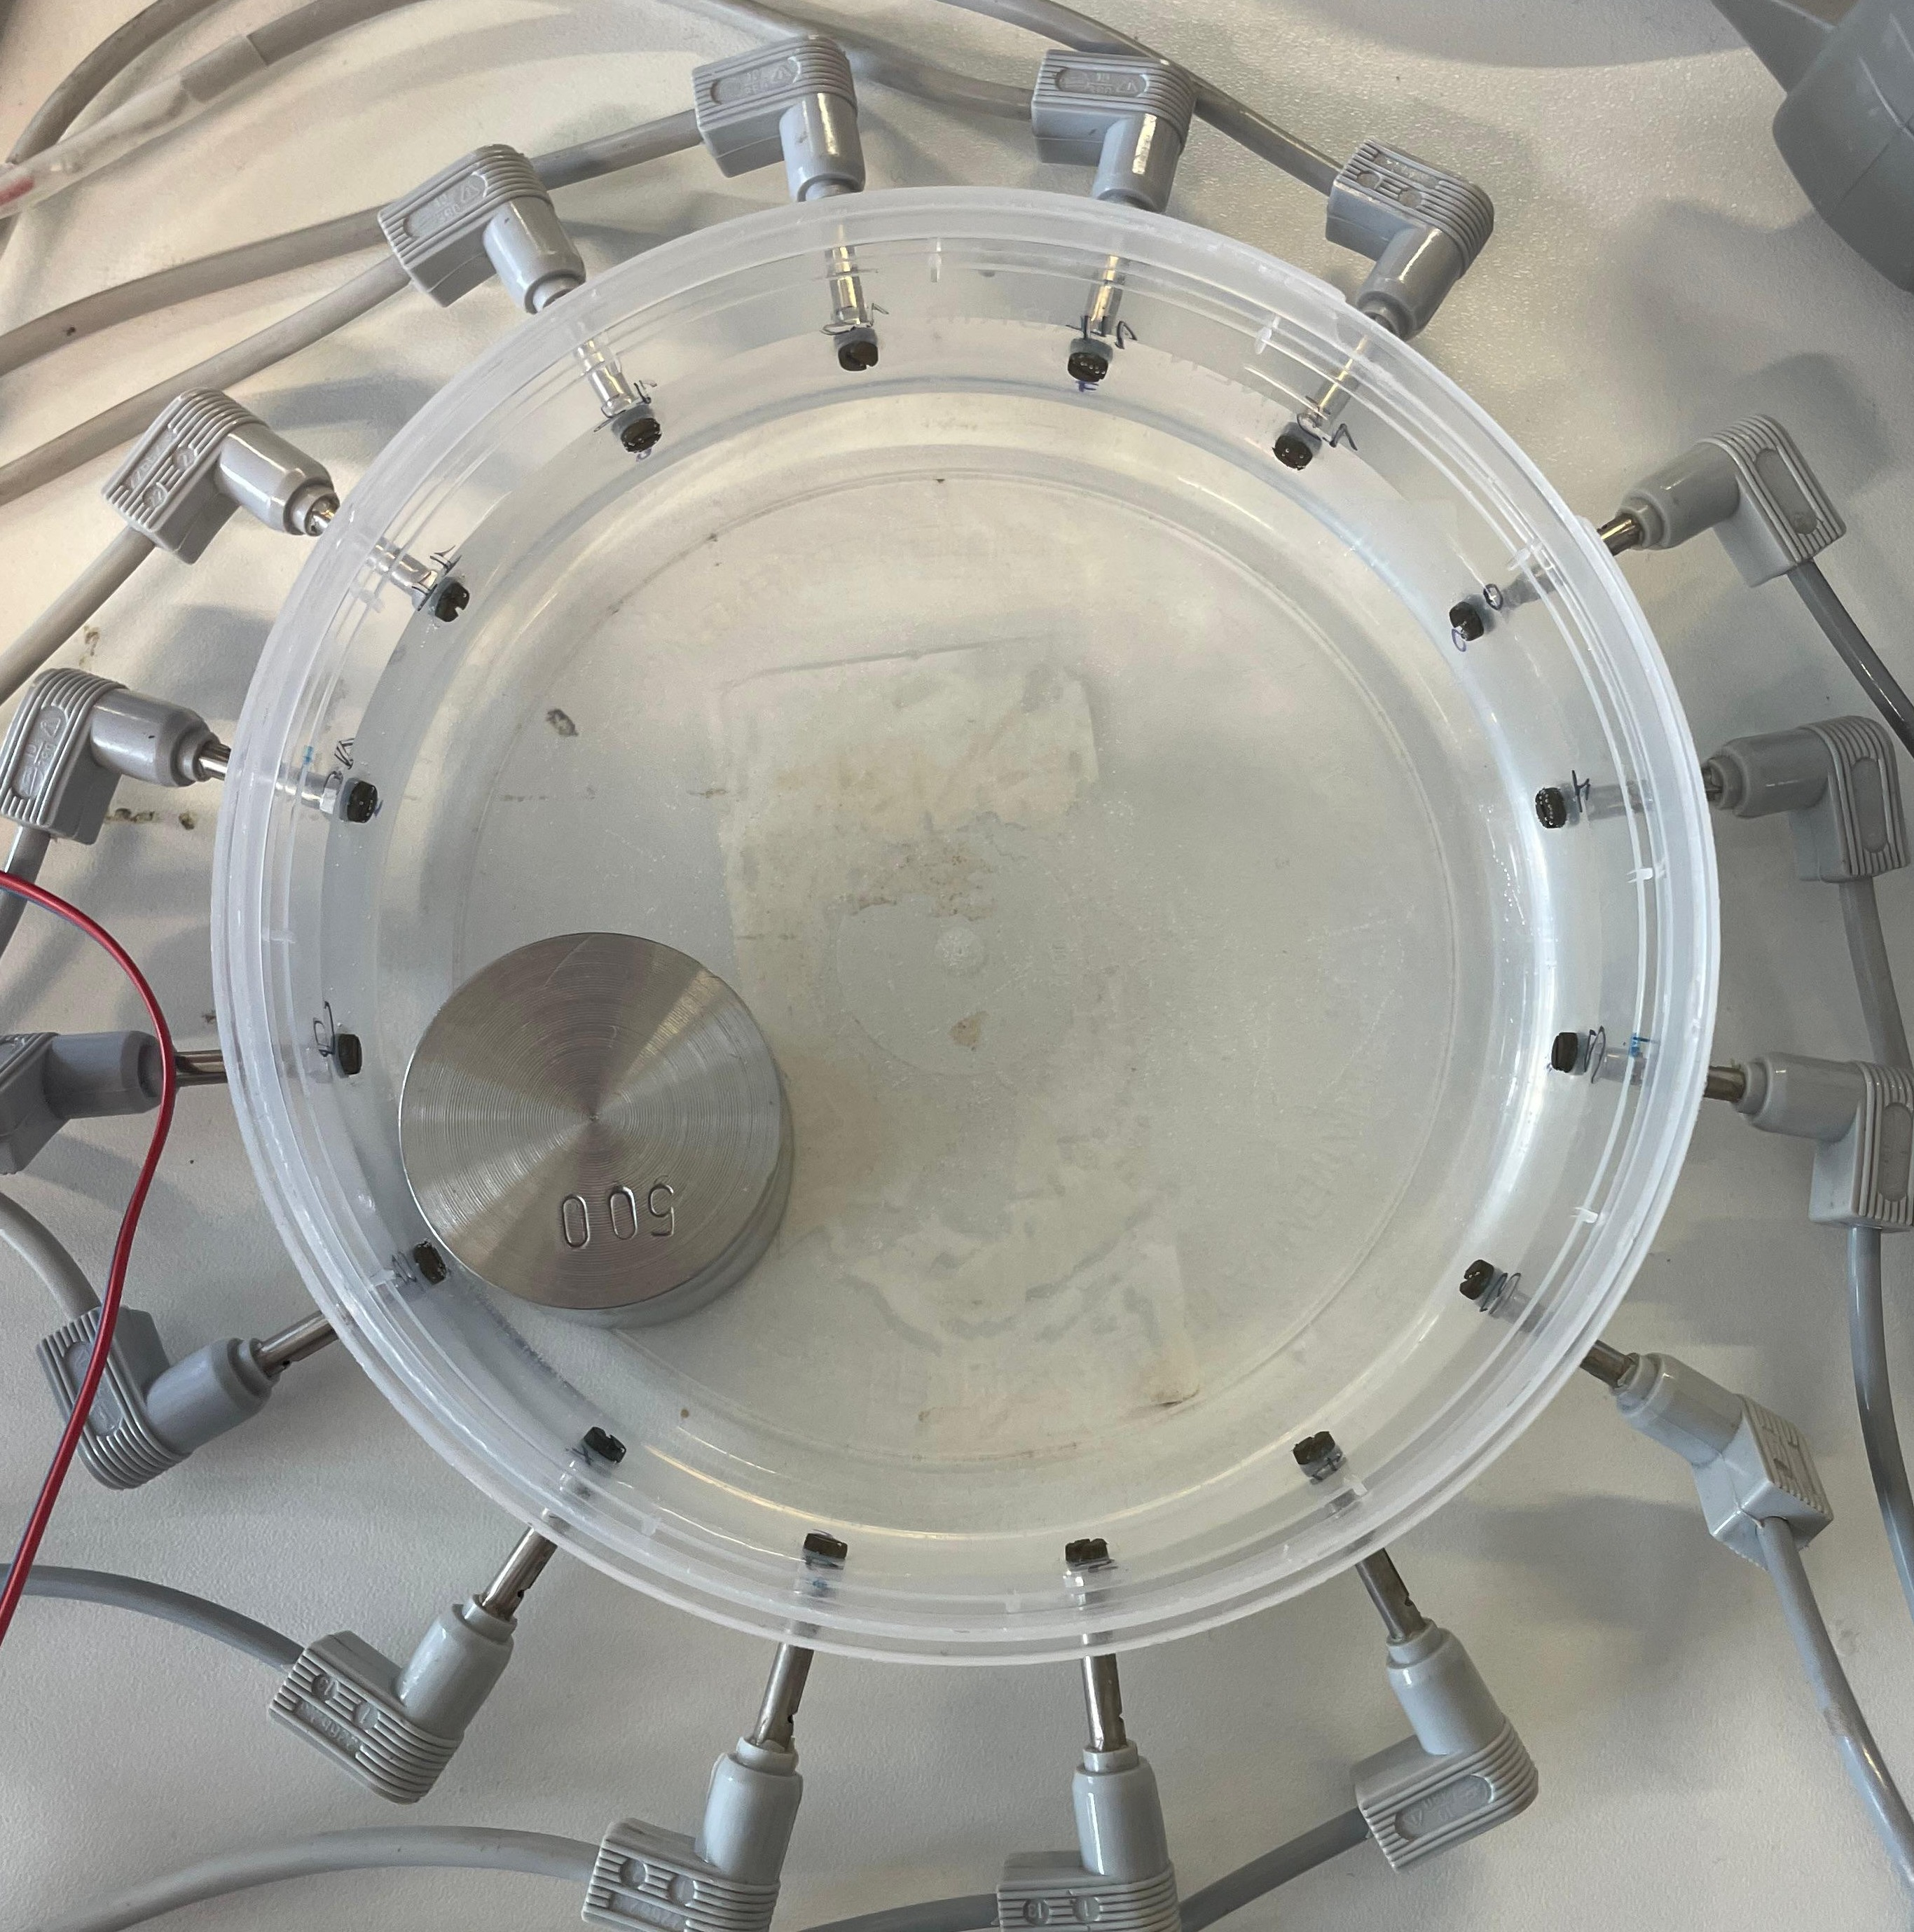
\includegraphics[width=\textwidth]{imagess/WhatsApp Image 2025-09-07 at 10.50.22_d7d43ed2.jpg} 
        \caption{Cylinder near electrode 0}
        \label{fig:cylinder_e0}
    \end{subfigure}
    \hspace{0.2\linewidth} % moderate space between images
    % Subfigure for position near electrode 7
    \begin{subfigure}[b]{0.31\linewidth}
        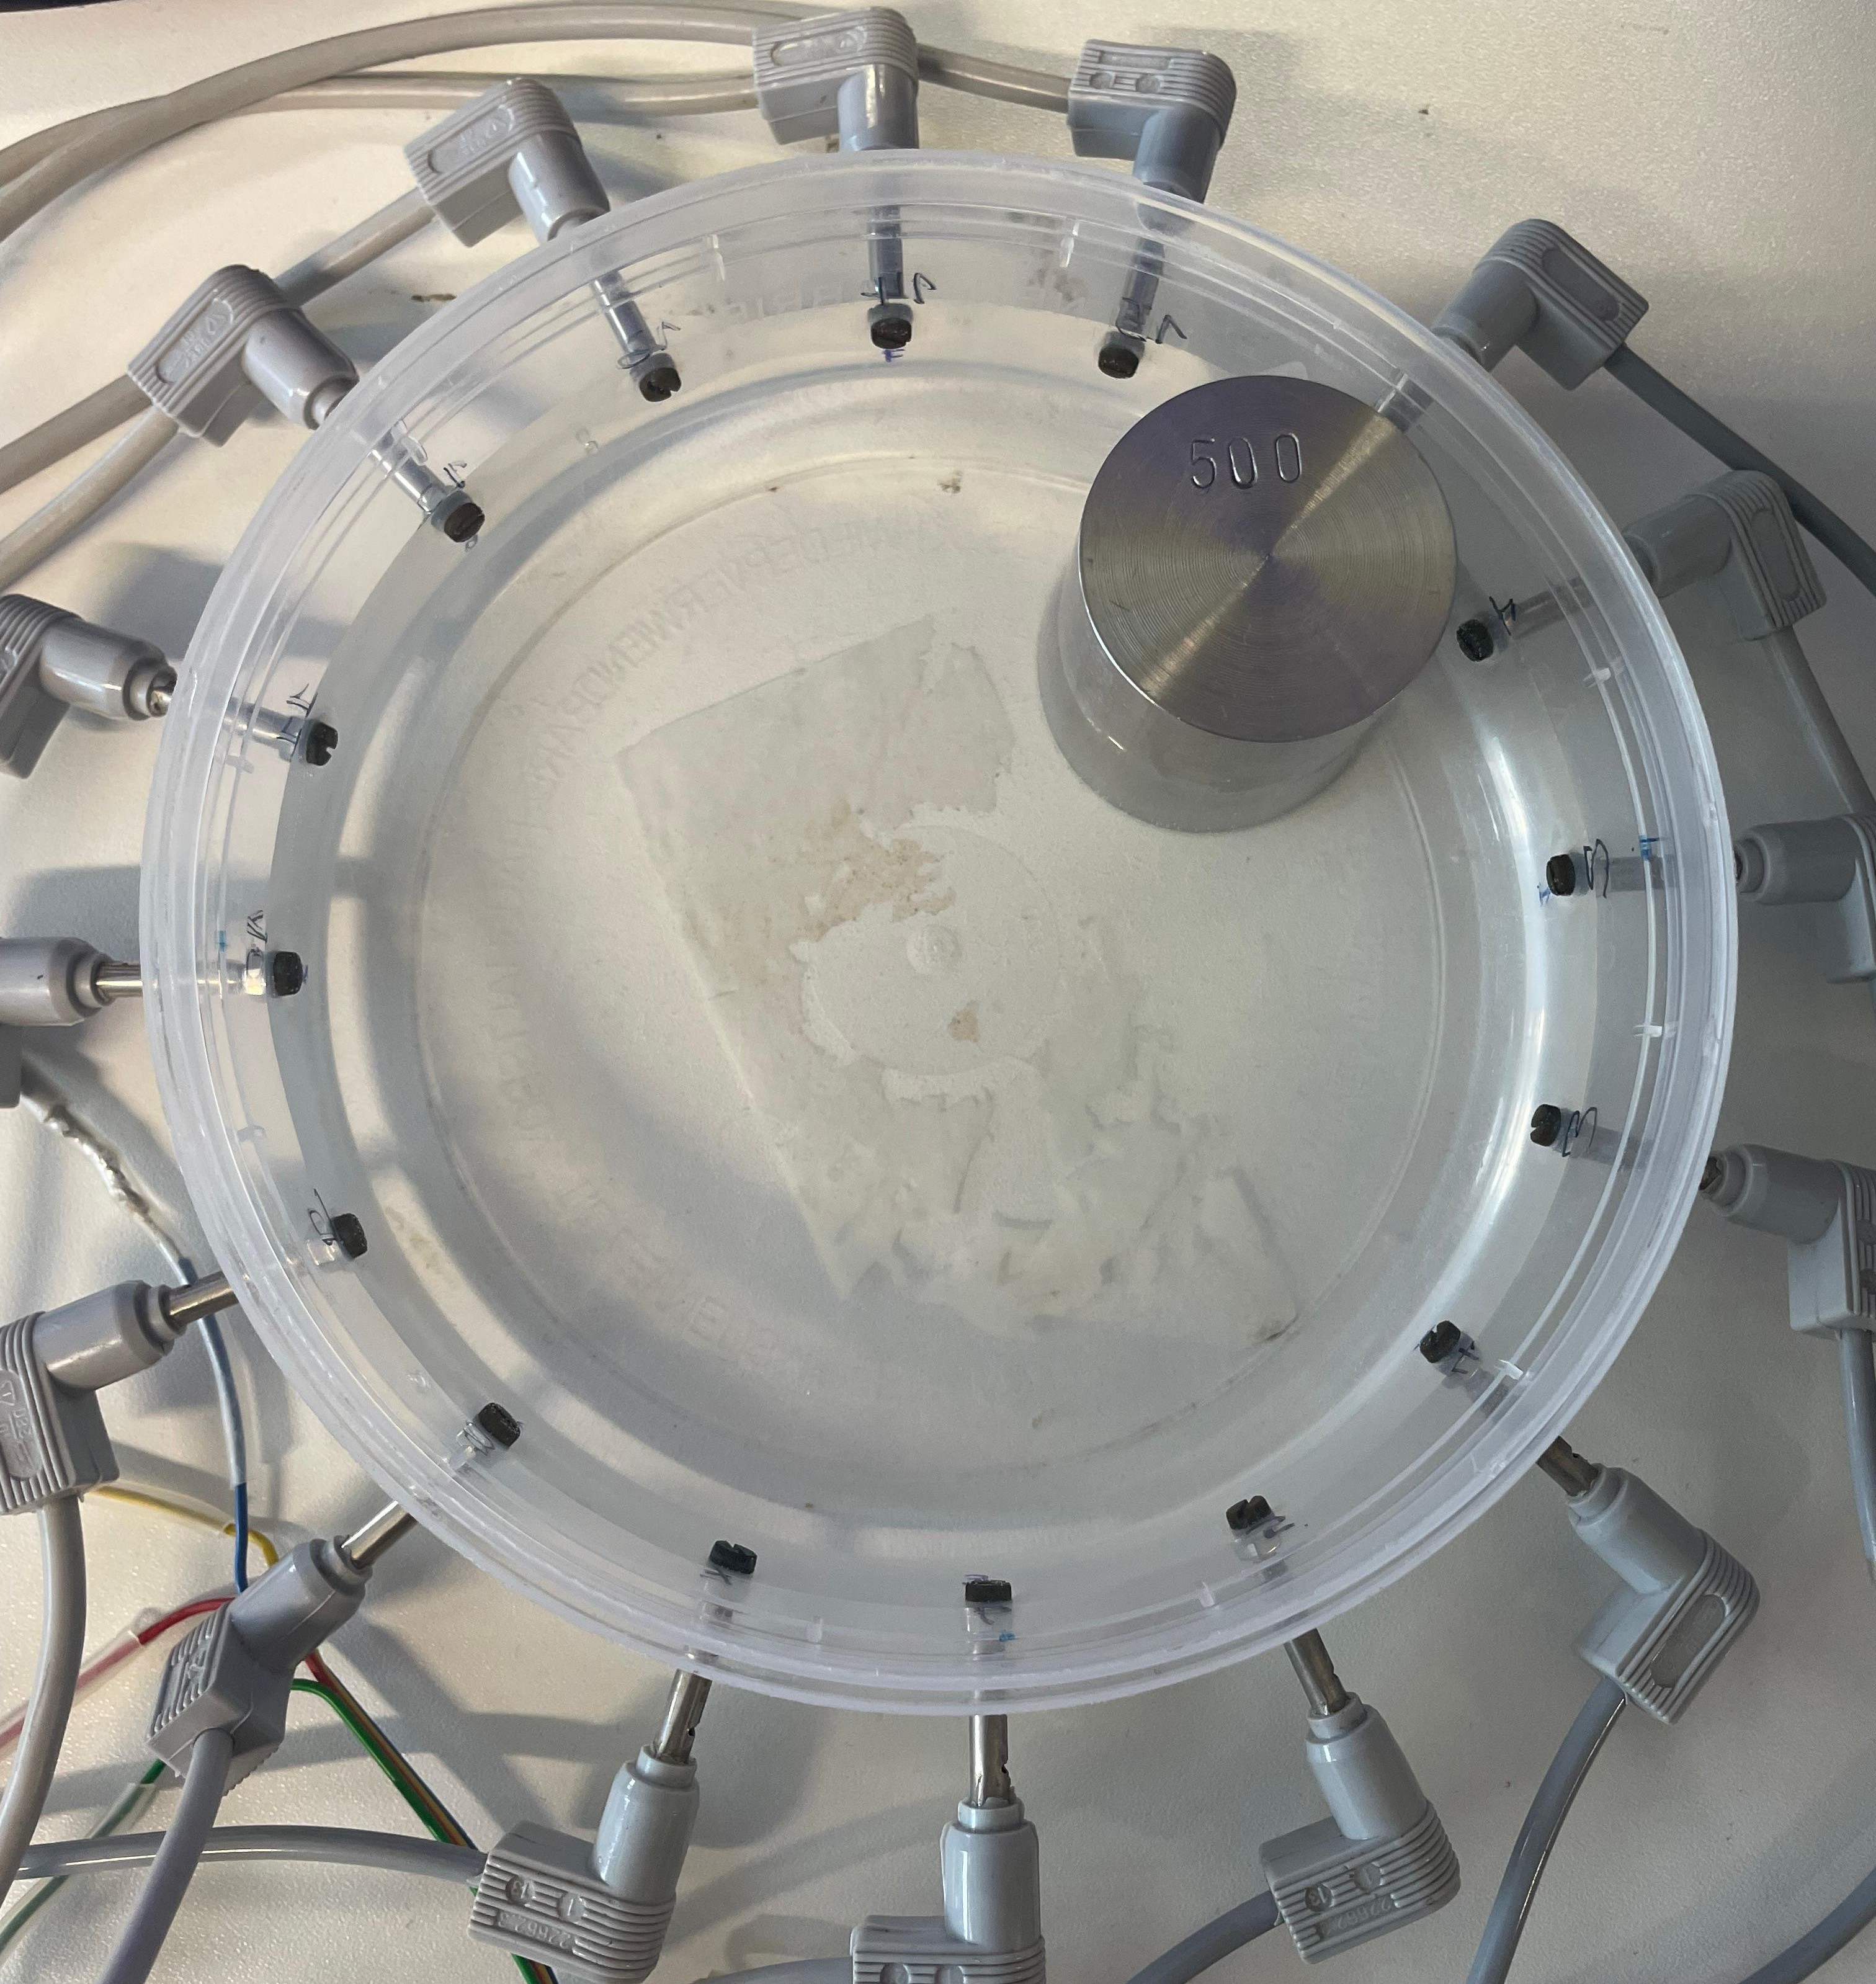
\includegraphics[width=\textwidth]{imagess/WhatsApp Image 2025-09-07 at 10.50.22_6e9b7119.jpg} 
        \caption{Cylinder near electrode 7}
        \label{fig:cylinder_e7}
    \end{subfigure}

    \caption{\footnotesize Experimental setup: water tank with a metallic cylindrical object in two different positions.}
    \label{fig:water_tank_setup_positions}
\end{figure}



  

% Explanatory sentence before the figure
Figure~\ref{fig:eit_recon_0} shows the reconstructed conductivity maps for a metallic object placed near electrode 0 
are shown below at two excitation frequencies.

\begin{figure}[H]
    \centering
    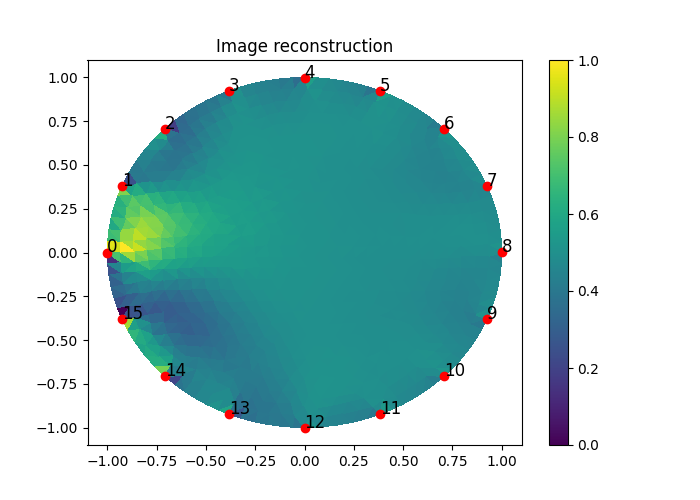
\includegraphics[width=0.45\linewidth]{imagess/figure0.png}
    \hfill
    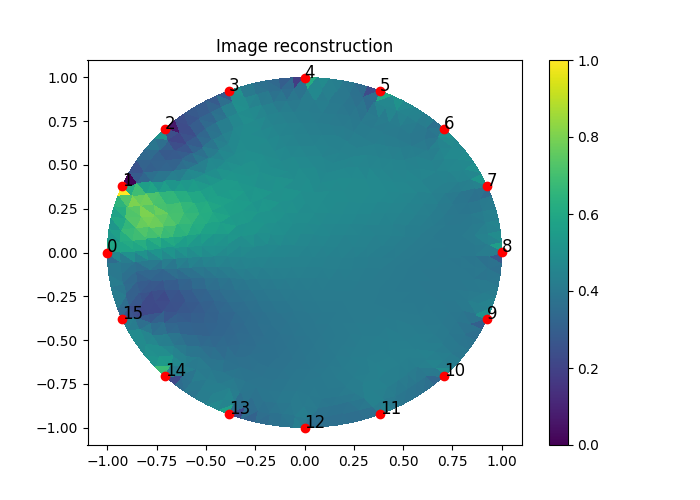
\includegraphics[width=0.45\linewidth]{imagess/Figure_44444444444444444.png}
    \caption{\footnotesize multi-frequency reconstructions of object near electrode 0: f = 9765.6250 kHz (left) and f = 49804.6875 kHz (right).}
    \label{fig:eit_recon_0}
\end{figure}

% Explanatory sentence before the figure
Figure~\ref{fig:eit_recon_7} reconstructed conductivity maps for a metallic object placed near electrode 7 
are shown below at two excitation frequencies.

\begin{figure}[H]
    \centering
    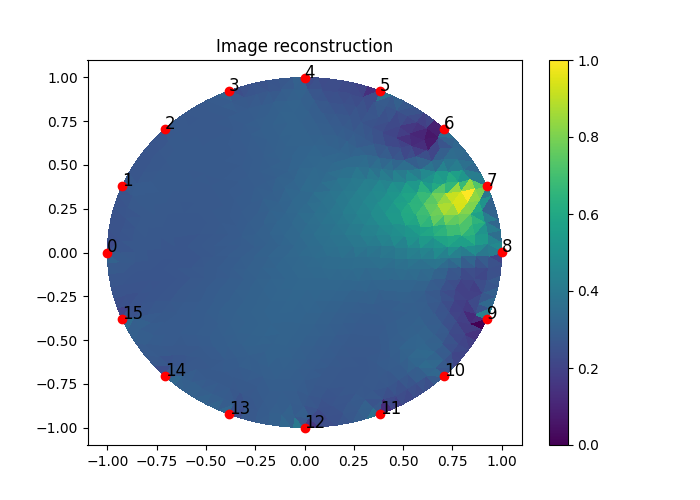
\includegraphics[width=0.45\linewidth]{imagess/electrode7777.png}
    \hfill
    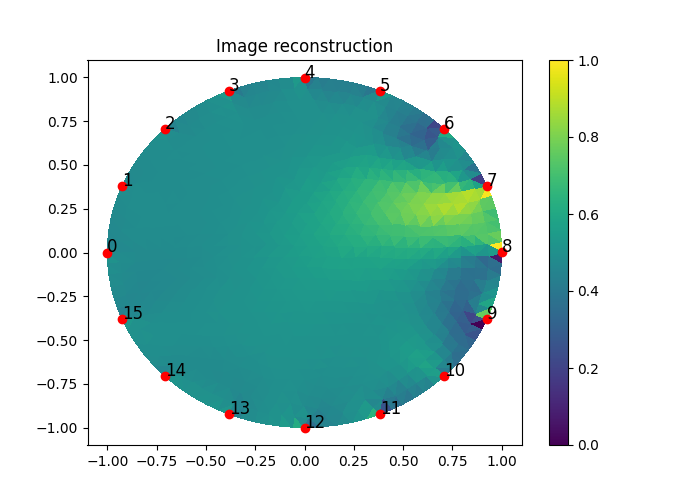
\includegraphics[width=0.45\linewidth]{imagess/electrode7.png}
    \caption{\footnotesize multi-frequency reconstructions of object near electrode 7: f = 9765.6250 kHz (left) and f = 49804.6875 kHz (right).}
    \label{fig:eit_recon_7}
\end{figure}

\subsubsection{Image reconstruction quality metrics}

Beyond visual inspection of the reconstructed conductivity maps, it is important to provide quantitative measures of image quality in order to assess the fidelity of the proposed system.

The Root Mean Squared Error (RMSE) can be computed between the reconstructed image and the reference experimental setup. This metric quantifies absolute pixel-level deviations and provides a direct measure of reconstruction accuracy\cite{adler2006uses}.

\begin{equation}
\text{RMSE} = \sqrt{\frac{1}{MN}\sum_{i=1}^{M}\sum_{j=1}^{N} \left(I_{ij}^{\text{recon}} - I_{ij}^{\text{ref}}\right)^2}
\end{equation}

The Signal-to-Noise Ratio (SNR) can be used also to evaluate the quality of the reconstructed image\cite{haase1991magnetic}:

\begin{equation}
\text{SNR} = \frac{\mu_{\text{signal}}}{\sigma_{\text{noise}}}
\end{equation}

These two metrics provide an objective basis to compare reconstructions across different experimental conditions and to evaluate the robustness of the imaging system.




\begin{table}[H]
\centering
\caption{Performance metrics for conductivity reconstruction at different positions and frequencies}
\label{tab:performance_metrics}
\begin{tabular}{|c|c|c|c|c|}
\hline
\textbf{Position} & \textbf{Electrode} & \textbf{Frequency (kHz)} & \textbf{RMSE} & \textbf{SNR (dB)} \\
\hline
Position 1 & Near Electrode 0 & 9765.6250 & $0.20$ & $28$ \\
\hline
Position 1 & Near Electrode 0 & 49804.6875 & $0.18$ & $32$ \\
\hline
Position 2 & Near Electrode 7 & 9765.6250 & $0.17$ & $22$ \\
\hline
Position 2 & Near Electrode 7 & 49804.6875 & $0.28$ & $32$ \\
\hline
\end{tabular}
\end{table}


\subsubsection{Multi-frequency EIT performance analysis}

Table~4.10 summarizes the performance metrics for conductivity reconstruction at two positions using low ($\sim 9.77$~kHz) and high ($\sim 49.8$~kHz) excitation frequencies. 
At the lower frequency, the Root Mean Squared Error (RMSE) is 0.20 near Electrode 0 (Position 1) and 0.17 near Electrode 7 (Position 2), with corresponding Signal-to-Noise Ratios (SNR) of 28~dB and 22~dB, respectively. 
Increasing the excitation frequency improves SNR across both positions (32~dB), indicating a stronger signal relative to measurement noise. 

These findings align with typical multi-frequency EIT behavior reported in the literature: higher excitation frequencies generally enhance signal quality but can lead to spatially non-uniform accuracy due to decreased sensitivity in regions distant from the electrodes. For instance, studies have shown that EIT systems operating at frequencies between 50 kHz and 250 kHz often achieve SNRs ranging from 25 dB to 35 dB, with RMSE values varying depending on the imaging protocol and system configuration which confirms the reliability and quality of the measurements.
\subsection{Experimental validation across 5 excitation frequencies}
Figure~\ref{fig:mf_reconstructions} presents the reconstructed images obtained after adjacent current injection in a water tank 
with a metallic cylindrical object placed near electrode 6 are shown below for 
five different excitation frequencies.
\begin{figure}[H]
    \centering
    % First row of images (3 images)
    \begin{subfigure}[b]{0.32\textwidth}
        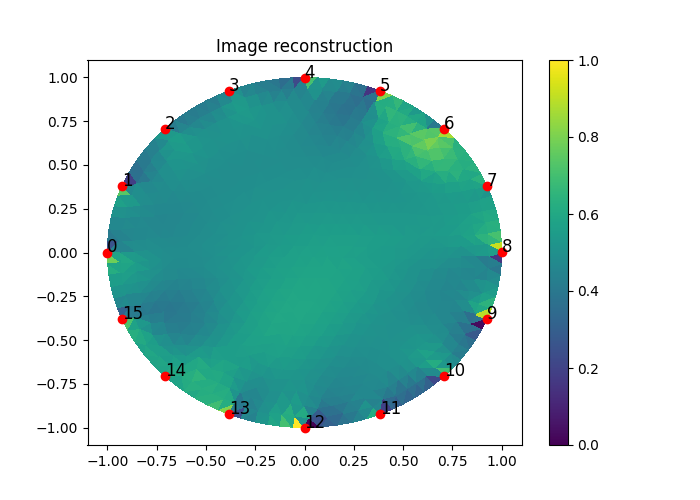
\includegraphics[width=\textwidth]{imagess/5f_3.png}
        \caption{Reconstruction at excitation frequency $f_1 = 9765.6250$ Hz}
    \end{subfigure}
    \hfill
    \begin{subfigure}[b]{0.32\textwidth}
        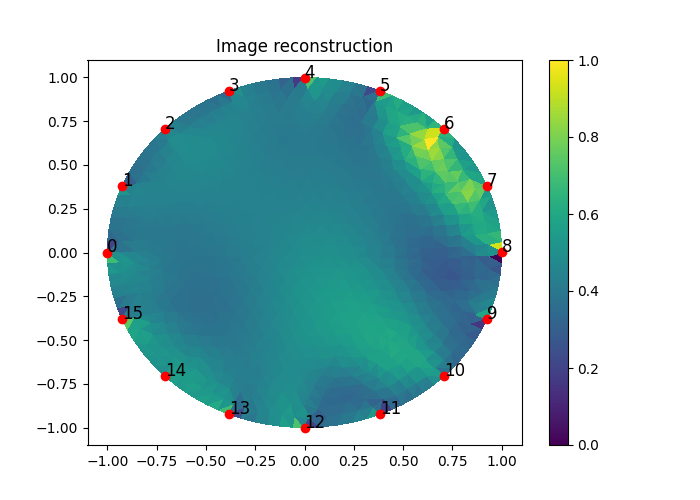
\includegraphics[width=\textwidth]{imagess/5f_2.png}
        \caption{Reconstruction at excitation frequency $f_2 = 22460.9375$ Hz}
    \end{subfigure}
    \hfill
    \begin{subfigure}[b]{0.32\textwidth}
        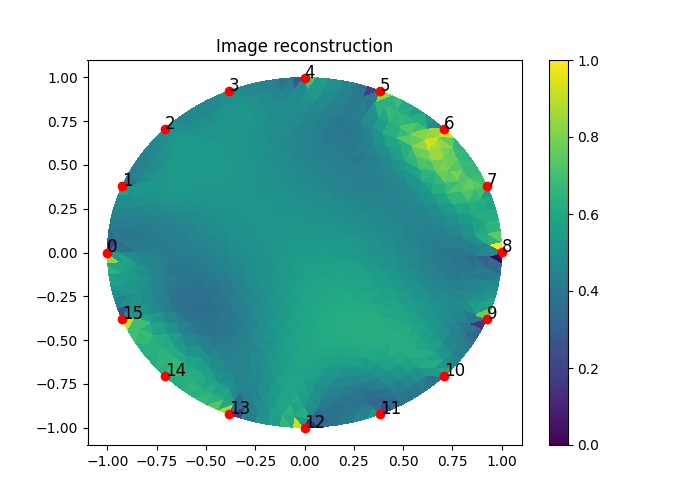
\includegraphics[width=\textwidth]{imagess/5f_1.png}
        \caption{Reconstruction at excitation frequency $f_3 = 49804.6875$ Hz}
    \end{subfigure}

    % Line break for second row
    \vskip\baselineskip

    % Second row of images (2 images, closer together)
    \begin{subfigure}[b]{0.32\textwidth}
        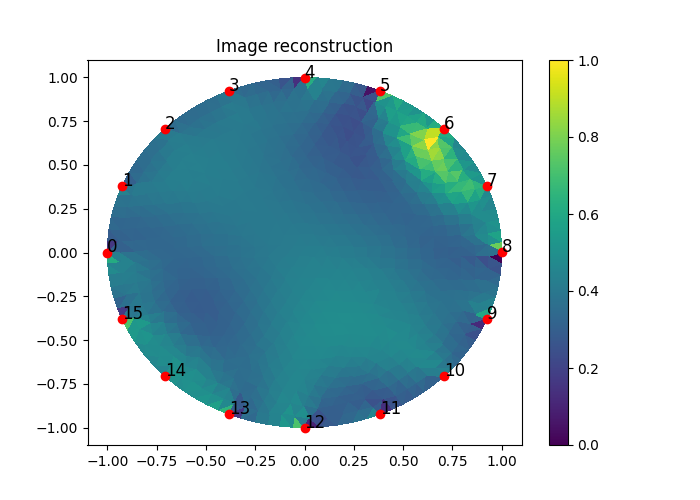
\includegraphics[width=\textwidth]{imagess/5f_4.png}
        \caption{Reconstruction at excitation frequency $f_4 = 111328.1250$ Hz}
    \end{subfigure}
    \hspace{1cm} % adjust this value for spacing between the two
    \begin{subfigure}[b]{0.32\textwidth}
        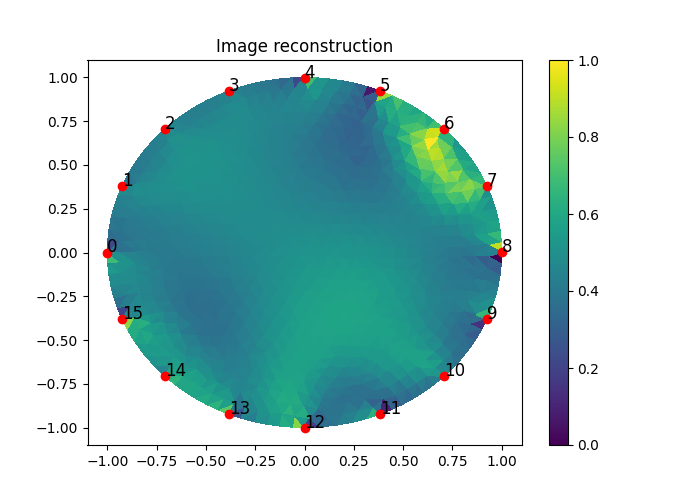
\includegraphics[width=\textwidth]{imagess/5f_5.png}
        \caption{Reconstruction at excitation frequency $f_5 = 250000.0000$ Hz}
    \end{subfigure}

    \caption{Multi-frequency reconstructions ($f_1$–$f_5$).}
    \label{fig:mf_reconstructions}
\end{figure}



As illustrated in Figure~\ref{fig:mf_reconstructions}, the reconstructed images correspond to the five excitation frequencies applied in the multi-frequency measurement. 
The metallic cylindrical object placed near electrode~6 is distinguishable in all reconstructions, appearing as a high-contrast region due to its significantly lower impedance compared to the surrounding saline water medium. 
However, the sharpness and localization of the reconstructed anomaly vary with frequency. At lower frequencies, the reconstructed object appears more diffused and less precisely localized, which can be attributed to the reduced sensitivity of adjacent current injection at low excitation frequencies. 
These results highlight the benefit of employing multi-frequency excitation for Electrical Impedance Tomography, as it provides complementary information across frequencies and allows for a more reliable identification of conductive inclusions in the imaging domain.\\
Although the metallic cylindrical object can be identified in the reconstructed images, the results are not perfectly accurate. 
The anomaly appears blurred and distorted, and its exact boundaries are difficult to delineate. 
This limitation can be mainly attributed to the intrinsic complexity of the EIT inverse problem, which is severely ill-posed and highly sensitive to modeling errors and measurement noise. 
Moreover, the use of multi-frequency excitation further increases the complexity of the reconstruction, since the tissue or medium response varies nonlinearly with frequency and requires accurate modeling of dispersive properties. The presence of boundary effects also reduces the achievable spatial resolution. 
As a result, while multi-frequency EIT provides complementary information, the reconstructions remain an approximation and must be interpreted with caution, highlighting the need for more advanced algorithms, better regularization strategies, and improved experimental setups to achieve higher fidelity images.




\section{Conclusion}
The frequency-domain measurements at an established resistance guaranteed that the EIT acquisition system yields stable and reproducible impedances over repeated trials. The experiment setup transferred this verification into the imaging domain. Reconstructed conductivity maps pinned down a metal object at different electrode positions and across multiple frequencies, showing the capability of the system to resolve spatial conductivity contrasts. Contrast between low- and high-frequency reconstructions is an indication of the complementary nature of multi-frequency excitation for higher image resolution and sensitivity.Overall, this chapter ensures the system built is stable in its impedance measurements and is capable of producing valid tomographic images, a sound foundation for further studies and uses of multi-frequency EIT.



